\graphicspath{{Chapters/TGCLimits/Figures/}}
\chapter{Limits on Anomalous Neutral Triple Gauge Couplings}
\label{chap:TGCLimits}

As discussed in~\sec{TheoryZZ-TGCs}, the presence of the anomalous neutral
triple gauge couplings (\TGC s), \ZZZ\ and \ZZg, present in some models of new
physics, would lead to an increase in the
\cx\ for \ZZ\ production, particularly at high momentum transfer. Observables
such as the mass of the four-lepton system and the transverse momenta of the \Z\
bosons and their decay products are therefore particularly sensitive to \TGC s.
The observed \ZZllll\ events are used to search for
such couplings, and in the absence of any evidence for them, to set limits on
the size of the couplings. The limits are obtained by performing a binned fit of
the \pt\ distribution of the leading \Z\ boson, although other variables are considered. Only
the \ZZ\ (on-shell) events are used. Separate limits are set using the 7~\tev\
and the 8~\tev\ data; for the 7~\tev\ analysis, limits are set in combination
with observed \ZZllvv\ events; see~\cite{ATLAS:2012kg} for a description of the
\ZZllvv\ analysis.

The limit setting procedure is described in~\sec{TGC-methodology}. A bin
optimisation study is presented in~\sec{TGC-BinOpt}, and the robustness of the
limits under variations in the limit setting method are described
in~\sec{TGC-Robustness}. Finally, the expected and observed limits are given
in~\sec{TGC-ExpObsLimits}.

\section{Limit Setting Procedure}
\label{sec:TGC-methodology}

In order to set limits it is necessary to parametrise the expected yield in
terms of the strength of the \TGC s. One method for doing this would be
to generate a grid of \mc\ samples at different coupling strengths. This is,
however, very computationally intensive. Instead, a matrix element reweighting procedure
is used to reweight a sample generated with one set of coupling strengths to another.
This is described in more detail below. Once the parameterised expected yields
are obtained, 95\% confidence interval limits on the \TGC s are set using a
frequentist likelihood-ratio method. This is also described below.

\subsection{Matrix Element Reweighting}
\label{sec:TGC-reweighting}

As described in~\sec{TheoryZZ-TGCs}, the anomalous \TGC s affecting \ZZ\
production are described by four parameters: \ffourg, \ffourZ, \ffiveg\ and
\ffiveZ.
Since the parameters enter linearly in the effective Lagrangian
(\eqn{tgc-lagrangian}), they will appear
quadratically in the amplitude for the \ZZllll\ process. The differential \cx\
can thus be written as:
\begin{eqnarray}\label{eqn:dsigma}
{\rm d}\sigma_{\rm SM+TGC} & = & F_{00} + f_4^\gamma F_{01} + f_4^Z F_{02} + f_5^\gamma F_{03} + f_5^Z F_{04}  \nonumber \\
&+& \left(f_4^\gamma\right)^2F_{11} + f_4^\gamma f_4^Z F_{12} +  f_4^\gamma f_5^\gamma F_{13} + f_4^\gamma f_5^Z F_{14}  \nonumber \\
&+& \left(f_4^Z\right)^2F_{22} + f_4^Zf_5^\gamma F_{23} + f_4^Zf_5^Z F_{24}  \nonumber \\
&+& \left(f_5^\gamma\right)^2F_{33} + f_5^\gamma f_5^Z F_{34} \nonumber \\
&+& \left(f_5^Z\right)^2F_{44}
\end{eqnarray}
where $F_{ij}$ are coefficients describing how the \cx\ changes in the presence
of \TGC s. A priori, there are 25 coefficients, however, using the 
symmetry property of the coefficients ($F_{ij}=F_{ji}$), it is seen 
that only $25-10=15$ are independent. $F_{00}$ corresponds to the contribution
of the \sm\ diagrams and the rest consist of operator contributions associated with the
anomalous couplings. 

A simulated event generated assuming only \sm\ couplings can be assigned a
weight corresponding to the increase in differential \cx\
due to \TGC s at a specific value of the four parameters:
\begin{equation}
{\rm weight} = \frac{{\rm d}\sigma_{\rm SM+TGC}(\ffourg, \ffourZ, \ffiveg,
\ffiveZ)}{{\rm d}\sigma_{\rm SM}}
\end{equation}
By assigning such a weight to every event in the sample, it is possible to reweight a sample
generated with only \sm\ couplings to a sample with \TGC s.
This procedure can be easily extended to reweight a sample generated assuming
any given set of \TGC s to any other set of \TGC s. For example, to reweight a sample
generated assuming only \sm\ couplings to sample assuming \ffourg=0.1, one would
apply to each event a weight:
\begin{eqnarray}\label{revisit}
{\rm weight} = \frac{F_{00} + 0.1 \cdot  F_{01} + (0.1)^{2} \cdot
F_{11}}{F_{00}}
\end{eqnarray}
The \Fij\ coefficients are completely specified by the kinematics of the
incoming and outgoing particles, and so must be evaluated on an event by event
basis. They are independent of the values of the anomalous coupling parameters
that the sample was generated assuming, although they do depend on the choice of
\formfactor. 

The coefficients are determined from the matrix elements for \ZZllll\
production in the presence of \TGC s, as follows. By using
Equation~\ref{eqn:dsigma} it is possible to write down 15 equations that
uniquely determine the coefficients $F_{ij}$ in terms of matrix elements
assuming particular values for the \TGC s.  To illustrate the procedure, it is
convenient to consider the simplified situation where there is just one coupling
parameter $f$.
In this case, there are 3 coefficients to be determined:
\begin{eqnarray}\label{revisit2}
{\rm d}\sigma_{\rm SM+TGC} = F_0 + fF_1 + f^2F_2 
\end{eqnarray}
where  $F_0={\rm d}\sigma_{\rm SM}$. Using three different values of $f$, e.g $f=\{0,1,-1\}$, three independent
equations may be written down:
\begin{eqnarray}\label{matrix1}
\left(\begin{array}{c}
{\rm d}\sigma_1\\
{\rm d}\sigma_2\\
{\rm d}\sigma_3
\end{array}\right) =
\left[\begin{array}{ccc}
1 & 0 & 0 \\
1 & 1 & 1 \\
1 & -1 & 1
\end{array}\right]
\left(\begin{array}{c}
F_0\\
F_1\\
F_2
\end{array}\right)
\end{eqnarray}
Denoting the matrix containing the coupling values $\hat{A}$, the \cx s
\dsigmavec\ and the coefficients $\vec{F}$, the equation may be
inverted to give the coefficients:
\begin{eqnarray}\label{matrix2} \dsigmavec=\hat{A}\vec{F} \qquad \Rightarrow \qquad \vec{F}=\hat{A}^{-1}{\rm
\bf d}\vec{\sigma} 
\end{eqnarray} 
This requires that $\hat{A}$ must be invertible. This is the
case if the coupling parameters are chosen such that the three equations in~\ref{matrix1}
are independent. When considering all four couplings at the same time, the
matrix $\hat{A}$ is 15$\times$15 and \dsigmavec\ and $\vec{F}$ are
15-dimensional vectors.

The \TGC\ matrix elements are obtained from the \BR\ code~\cite{Baur:2000ae};
matrix elements from the \BHO~\cite{bho} code are also used as a cross-check. 
%The \TGC\ matrix elements are obtained from the next-to-leading order \mc\
%generator \BHO~\cite{bho}. Matrix elements from the leading-order \BR\
%generator~\cite{Baur:1994au} are also used as a cross-check. 
The matrix
elements are introduced into the  framework described in~\cite{Bella:2008wc},
which enables a calculation of the amplitude given the four-vectors and PDG
codes of the incoming partons and outgoing particles from the hard process. 

Whilst it is possible to reweight a \sm\ sample to an \TGC\ point, this suffers
from a lack of statistics in the tails of distributions such as the \Z\ boson
\pt\ and the four-lepton invariant mass, which are the regions of greatest
interest when studying \TGC s. Instead, samples generated with values of the
\TGC parameters set near previously derived experimental limits are used; this
ensures statistics in the tails of the distributions of interest. The
\powhegbox\ and \ggZZ\ generators used to generate the nominal signal samples do
not model \TGC s; instead the samples are generated using \sherpa, which does.
For the 7~\tev\ analysis, four samples are used, with couplings
$\{f_{4}^{\gamma}=0.1\}$, $\{f_{5}^{\gamma}=-0.1\}$, $\{f_{4}^{\gamma}=0.1$ \&
$f_{5}^{\gamma}=0.1\}$, and $\{f_{4}^{Z}=0.1$ \& $f_5^{Z}=0.1\}$. For the
8~\tev\ analysis, three sample are used, with couplings $\{\ffourg=0.1\}$
(denoted TGC0), $\{\ffourg=0.1 \,\&\, \ffiveZ=0.1\}$ (denoted TGC1), and $\{
\ffourg = \ffourZ = \ffiveg = \ffiveZ = 0.1 \}$ (denoted TGC2). The 7~\tev\
samples are generated with a \formfactor\ of $\Lambda=2\tev,n=3$; the 8~\tev\
samples are generated without a \formfactor. The reweighting procedure can be
used to reweight samples generated with one choice of \formfactor\ (or no
\formfactor) to another choice of \formfactor.

\subsection{Validation of Reweighting Procedure}
\label{sec:TGC-ReweightingValidation}

To demonstrate the performance of the reweighting procedure, the 8~\tev\
\sherpa\ samples generated with \TGC s are reweighted to the \sm, and compared
to a sample generated assuming only \sm\ couplings. Additionally, the TGC1 and
TGC2 samples are reweighted to the TGC0 sample. \fig{TGC-reweight} shows the
resulting distributions of the leading \Z\ boson \pt, and the ratios of the
reweighted samples to the \sm/TGC0 distribution, for reweighting carried out
using either the \BHO\ or the \BR\ matrix elements. For both of the codes, the
reweighted samples are seen to agree well with the directly generated samples.

\begin{figure}[htbp]
\begin{center}
\subfigure[\BR]{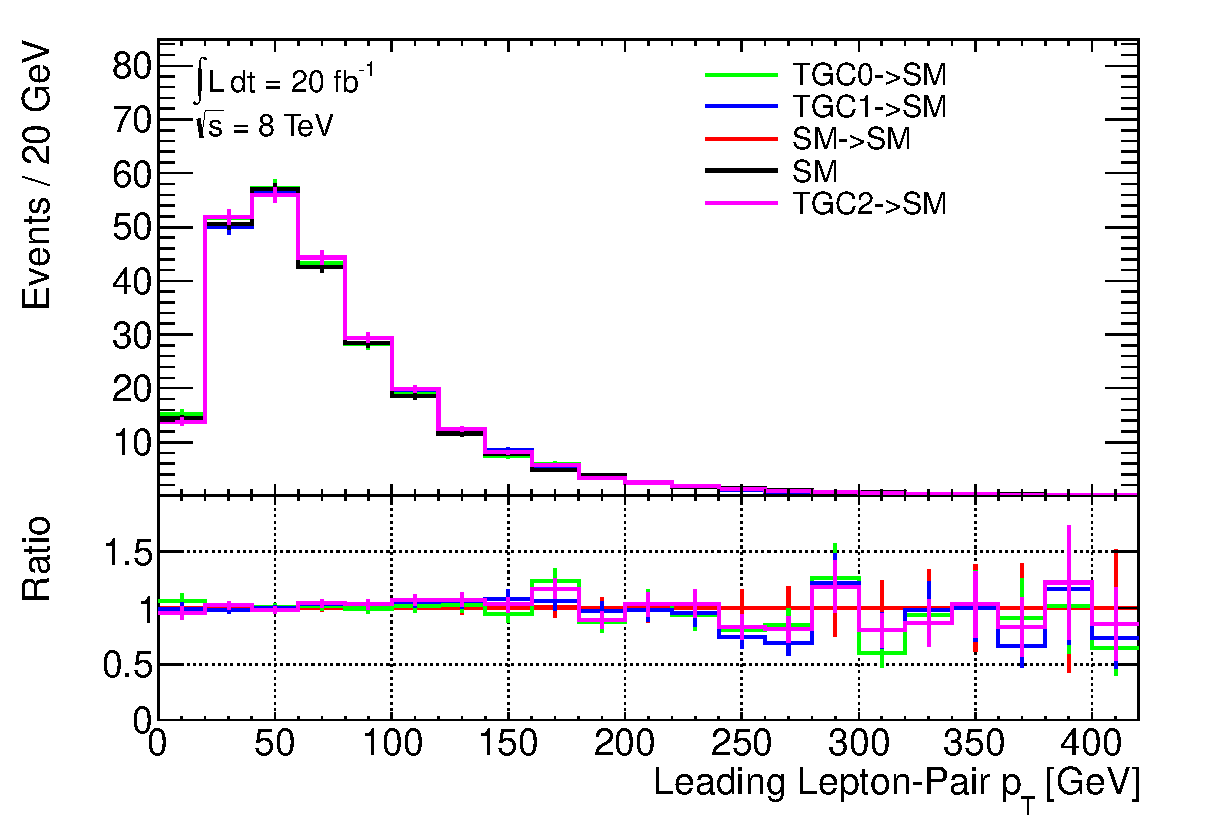
\includegraphics[width=0.47\textwidth]{ReweightValidation/04_BR/ZZ_Z1_pt_sm}}
\subfigure[\BHO]{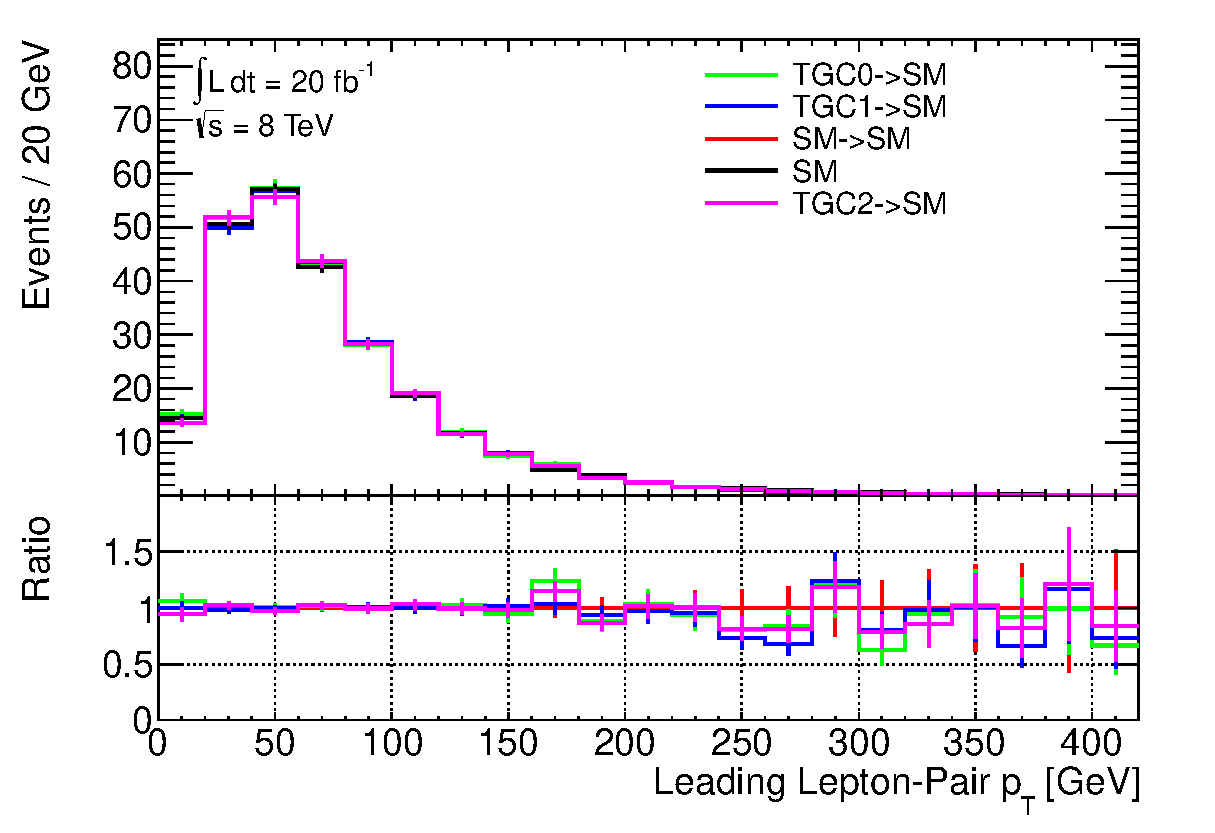
\includegraphics[width=0.47\textwidth]{ReweightValidation/04_BHO_noFF/ZZ_Z1_pt_sm}}
\subfigure[\BR]{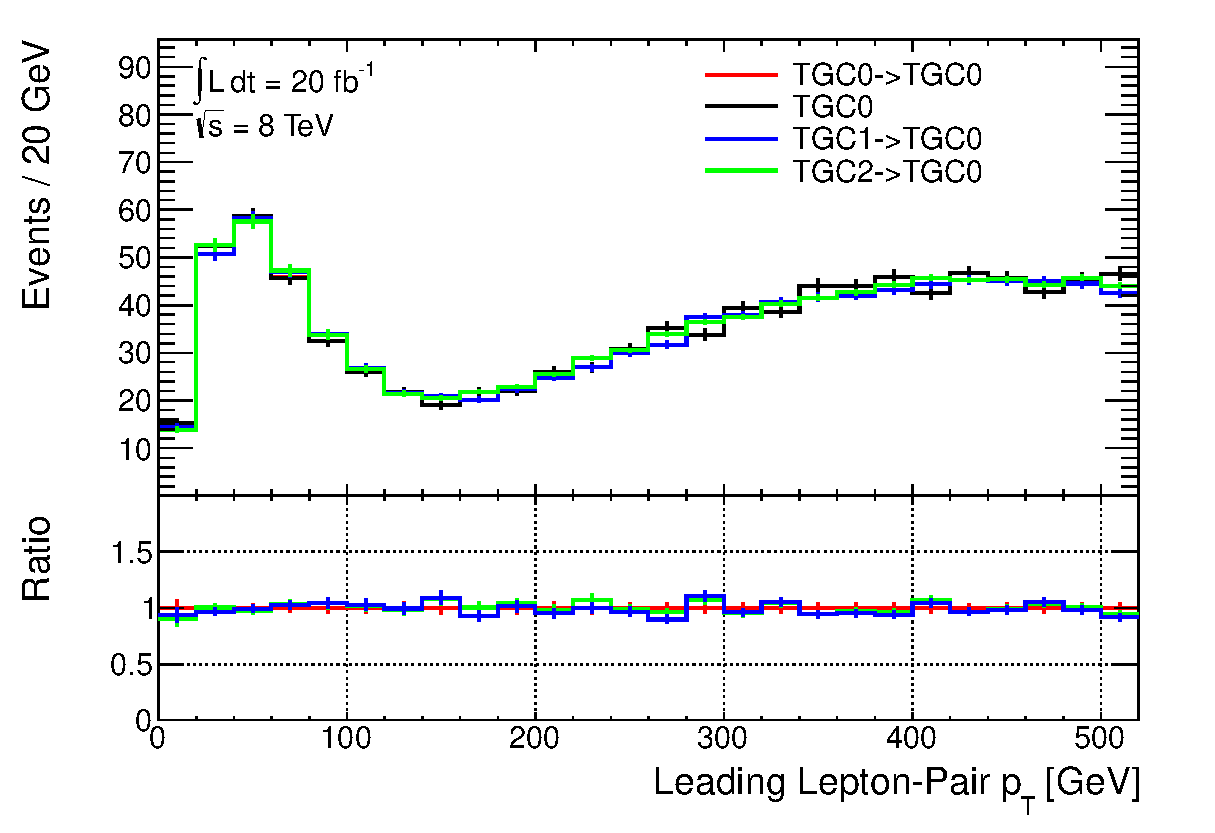
\includegraphics[width=0.47\textwidth]{ReweightValidation/04_BR/ZZ_Z1_pt_tgc0}}
\subfigure[\BHO]{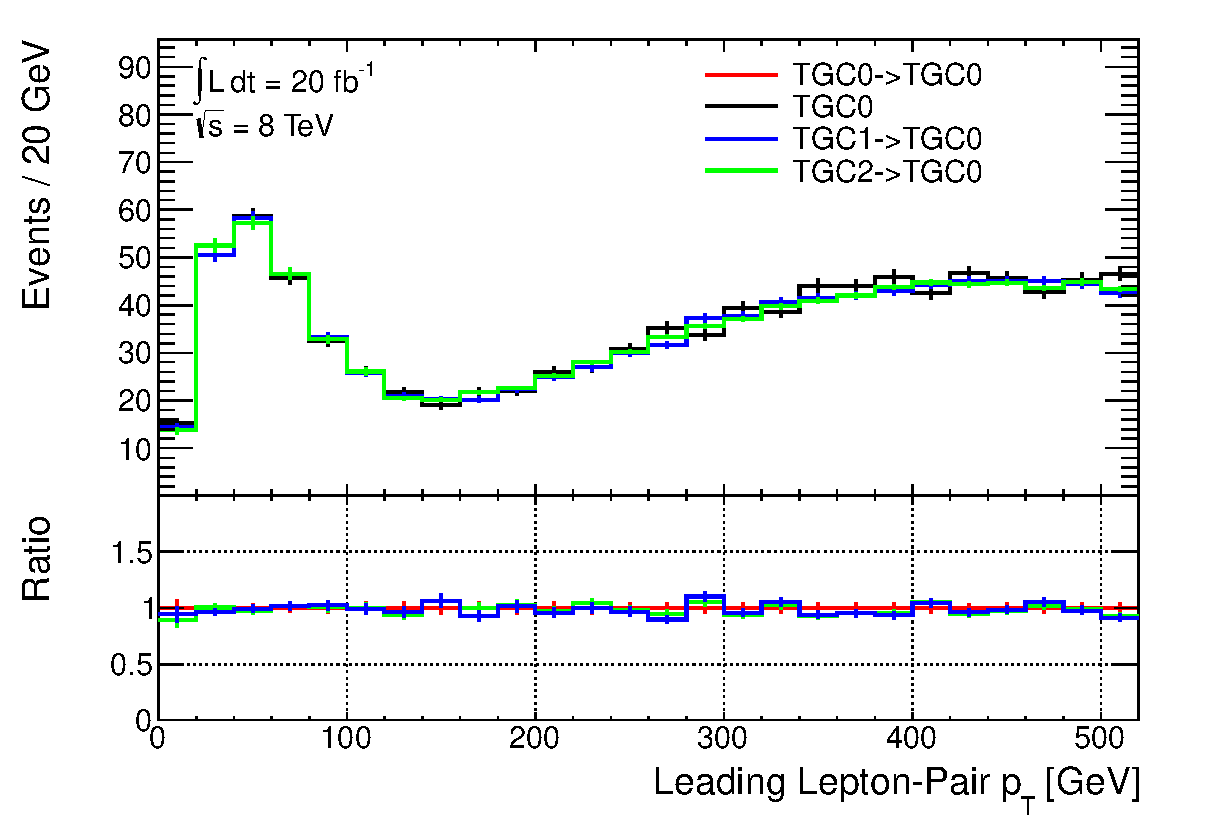
\includegraphics[width=0.47\textwidth]{ReweightValidation/04_BHO_noFF/ZZ_Z1_pt_tgc0}}
\caption[Validation of the TGC reweighting procedure for the 8~\tev\ samples.]{
\small
Validation of the TGC reweighting procedure for the 8~\tev\ samples. Figures (a) and (b) show the \pt\
distribution of the leading \leppair, showing the three \TGC\ samples (TGC0,
TGC1, TGC2; green, blue and pink lines) generated with different couplings and
the \sm\ sample (red line), reweighted to the \sm\
expectation using the procedure described in~\sec{TGC-reweighting}, compared to the sample
generated assuming only \sm\ couplings (SM, black line). In Figure (a) the matrix elements
of the \BR\ code are used, and in Figure (b) the matrix elements of
the \BHO\ code are used. Figures (c) and (d) show the same distribution,
showing the TGC0, TGC1 and TGC2 samples (red, blue and green lines) reweighted to the TGC0 \TGC\ point
($\ffourg=0.1$) compared to the non-reweighted TGC0 sample (black line).
 }
\label{fig:TGC-reweight}
\end{center}
\end{figure}

\subsection{Yield Coefficients}
\label{sec:TGC-YieldCoefficients}

In order to extract limits on the \TGC s, an estimate of the number of expected
events passing the selection requirements as a
function of the \TGC\ parameters must be obtained. The expect yield is parameterised by
yield coefficients \Yij, which are be obtained from the \Fij\ as:
\begin{equation}
\Yij = \left( \sum_{\rm events} \frac{F_{ij}}{F_{00} } \right) \cdot{N_{\rm expected}}.
\end{equation}
where $N_{\rm expected}$ is the \sm\ number of expected events, obtained from the
nominal signal sample, and the sum is over events passing the full event
selection. Event-level lepton selection efficiency, energy scale, and resolution corrections
are taken into account when calculating the yield coefficients. A different set of yield
coefficients is needed for each bin of the differential distribution used to set
the limits and for each choice of
form-factor. The expected yield as a function of the \TGC\ parameters is given by
\begin{eqnarray}\label{eqn:Nexp_TGC}
N_{exp} (\ffourg, \ffourZ, \ffiveg, \ffiveZ) & = & Y_{00} + f_4^\gamma Y_{01} + f_4^Z Y_{02} + f_5^\gamma Y_{03} + f_5^Z Y_{04}  \nonumber \\
&+& \left(f_4^\gamma\right)^2Y_{11} + f_4^\gamma f_4^Z Y_{12} +  f_4^\gamma f_5^\gamma Y_{13} + f_4^\gamma f_5^Z Y_{14}  \nonumber \\
&+& \left(f_4^Z\right)^2Y_{22} + f_4^Zf_5^\gamma Y_{23} + f_4^Zf_5^Z Y_{24}  \nonumber \\
&+& \left(f_5^\gamma\right)^2Y_{33} + f_5^\gamma f_5^Z Y_{34} \nonumber \\
&+& \left(f_5^Z\right)^2Y_{44}
\end{eqnarray}

%\tabs{TGC-yieldCoeffs-seven-n3L3}{TGC-yieldCoeffs-seven-noFF} shows the yield
%coefficients for the 7~\tev\ analysis for the total number of events case with a \formfactor\
%of $\Lambda=3~\tev, n=3$ and for the case of no \formfactor.
%\tabs{TGC-yieldCoeffs-eight-n3L3}{TGC-yieldCoeffs-eight-noFF} shows the
%equivalent coefficients for the 8~\tev\ analysis. In all cases, these are
%obtained from the \BR\ generator using the TGC0 sample. 
\tabs{TGC-yieldCoeffs-eight-n3L3}{TGC-yieldCoeffs-eight-noFF} show the yield
coefficients for the 8~\tev\ analysis for the total number of events case with a
\formfactor\ of $\Lambda=3~\tev, n=3$ and for the case of no \formfactor,
obtained using the \BR\ matrix-elements to reweight the TGC0 sample.  \fig{TGC-yield-curves}
shows the expected total event yield for the 8~\tev\ analysis as a function of
the four \TGC\ parameters. In each case, the parameters not being varied are
assumed to be at their \sm\ values of zero.
The solid blue curve shows the yields with a \formfactor\ of $n=3, \Lambda=3~\tev$;
the dashed red curve shows the yields with no \formfactor. The increase of event
yield with the strength of the coupling is reduced as a result of applying the
\formfactor.

%The yield coefficients for each bin of
%the differential distributions are shown in Appendix~\ref{appendix:tgc-coeff}. 
%
%\begin{table}[htbp]
%\small
%\centering
%\begin{tabular}{lcccc}
%\hline\hline
%       $Y_{SM}$ &             $Y_{\ffourg}$ &             $Y_{\ffourZ}$ &             $Y_{\ffiveg}$ &             $Y_{\ffiveZ}$ \\
%292.5 $\pm$ 3.1 &             1.1 $\pm$ 2.3 &            -9.6 $\pm$ 5.0 &            12.4 $\pm$ 2.5 &            -7.8 $\pm$ 5.9 \\
%\hline
%                &  $Y_{\ffourg}Y_{\ffourg}$ &  $Y_{\ffourg}Y_{\ffourZ}$ &  $Y_{\ffourg}Y_{\ffiveg}$ &  $Y_{\ffourg}Y_{\ffiveZ}$ \\
%                &      146439.4 $\pm$ 827.9 &      130911.0 $\pm$ 871.3 &         -79.8 $\pm$ 181.2 &         -74.9 $\pm$ 100.7 \\
%\hline
%                &  $Y_{\ffourZ}Y_{\ffourZ}$ &  $Y_{\ffourZ}Y_{\ffiveg}$ &  $Y_{\ffourZ}Y_{\ffiveZ}$ \\
%                &     197589.1 $\pm$ 1480.2 &         -75.2 $\pm$ 100.7 &        -213.1 $\pm$ 323.4 \\
%\hline
%                &  $Y_{\ffiveg}Y_{\ffiveg}$ &  $Y_{\ffiveg}Y_{\ffiveZ}$ \\
%                &      143338.6 $\pm$ 837.1 &      127865.4 $\pm$ 879.3 \\
%\hline
%                &  $Y_{\ffiveZ}Y_{\ffiveZ}$ \\
%                &     192851.2 $\pm$ 1492.7 \\
%\hline\hline
%\end{tabular}
%\caption{Yield coefficients for the 7~\tev\ analysis with \formfactor\ $n=3, \Lambda=3~\tev$.}
%\label{table:TGC-yieldCoeffs-seven-n3L3}
%\end{table}
%
%\begin{table}[htbp]
%\small
%\centering
%\begin{tabular}{lcccc}
%\hline\hline
%       $Y_{SM}$ &             $Y_{\ffourg}$ &             $Y_{\ffourZ}$ &             $Y_{\ffiveg}$ &             $Y_{\ffiveZ}$ \\
%292.5 $\pm$ 3.1 &             0.6 $\pm$ 2.1 &            -9.0 $\pm$ 4.6 &            11.1 $\pm$ 2.4 &            -7.4 $\pm$ 5.5 \\
%\hline
%                &  $Y_{\ffourg}Y_{\ffourg}$ &  $Y_{\ffourg}Y_{\ffourZ}$ &  $Y_{\ffourg}Y_{\ffiveg}$ &  $Y_{\ffourg}Y_{\ffiveZ}$ \\
%                &       51241.3 $\pm$ 335.4 &       47083.3 $\pm$ 364.1 &           21.8 $\pm$ 85.6 &           21.0 $\pm$ 46.8 \\
%\hline
%                &  $Y_{\ffourZ}Y_{\ffourZ}$ &  $Y_{\ffourZ}Y_{\ffiveg}$ &  $Y_{\ffourZ}Y_{\ffiveZ}$ \\
%                &       71922.3 $\pm$ 624.8 &           20.8 $\pm$ 46.8 &          60.9 $\pm$ 153.6 \\
%\hline
%                &  $Y_{\ffiveg}Y_{\ffiveg}$ &  $Y_{\ffiveg}Y_{\ffiveZ}$ \\
%                &       49311.1 $\pm$ 336.1 &       45165.5 $\pm$ 363.4 \\
%\hline
%                &  $Y_{\ffiveZ}Y_{\ffiveZ}$ \\
%                &       68920.8 $\pm$ 623.2 \\
%\hline\hline
%\end{tabular}
%\caption{Yield coefficients for the 7~\tev\ analysis with no \formfactor.}
%\label{table:TGC-yieldCoeffs-seven-noFF}
%\end{table}

\begin{table}[htbp]
\small
\centering
\begin{tabular}{lcccc}
\hline\hline
       $Y_{SM}$ &             $Y_{\ffourg}$ &             $Y_{\ffourZ}$ &             $Y_{\ffiveg}$ &             $Y_{\ffiveZ}$ \\
292.5 $\pm$ 3.1 &             1.1 $\pm$ 2.3 &            -9.6 $\pm$ 5.0 &            12.4 $\pm$ 2.5 &            -7.8 $\pm$ 5.9 \\
\hline
                &  $Y_{\ffourg}Y_{\ffourg}$ &  $Y_{\ffourg}Y_{\ffourZ}$ &  $Y_{\ffourg}Y_{\ffiveg}$ &  $Y_{\ffourg}Y_{\ffiveZ}$ \\
                &      146439.4 $\pm$ 827.9 &      130911.0 $\pm$ 871.3 &         -79.8 $\pm$ 181.2 &         -74.9 $\pm$ 100.7 \\
\hline
                &  $Y_{\ffourZ}Y_{\ffourZ}$ &  $Y_{\ffourZ}Y_{\ffiveg}$ &  $Y_{\ffourZ}Y_{\ffiveZ}$ \\
                &     197589.1 $\pm$ 1480.2 &         -75.2 $\pm$ 100.7 &        -213.1 $\pm$ 323.4 \\
\hline
                &  $Y_{\ffiveg}Y_{\ffiveg}$ &  $Y_{\ffiveg}Y_{\ffiveZ}$ \\
                &      143338.6 $\pm$ 837.1 &      127865.4 $\pm$ 879.3 \\
\hline
                &  $Y_{\ffiveZ}Y_{\ffiveZ}$ \\
                &     192851.2 $\pm$ 1492.7 \\
\hline\hline
\end{tabular}
\caption{Yield coefficients for the 8~\tev\ analysis with \formfactor\ $n=3, \Lambda=3~\tev$.}
\label{table:TGC-yieldCoeffs-eight-n3L3}
\end{table}

\begin{table}[htbp]
\small
\centering
\begin{tabular}{lcccc}
\hline\hline
       $Y_{SM}$ &             $Y_{\ffourg}$ &             $Y_{\ffourZ}$ &             $Y_{\ffiveg}$ &             $Y_{\ffiveZ}$ \\
292.5 $\pm$ 3.1 &             0.6 $\pm$ 2.1 &            -9.0 $\pm$ 4.6 &            11.1 $\pm$ 2.4 &            -7.4 $\pm$ 5.5 \\
\hline
                &  $Y_{\ffourg}Y_{\ffourg}$ &  $Y_{\ffourg}Y_{\ffourZ}$ &  $Y_{\ffourg}Y_{\ffiveg}$ &  $Y_{\ffourg}Y_{\ffiveZ}$ \\
                &       51241.3 $\pm$ 335.4 &       47083.3 $\pm$ 364.1 &           21.8 $\pm$ 85.6 &           21.0 $\pm$ 46.8 \\
\hline
                &  $Y_{\ffourZ}Y_{\ffourZ}$ &  $Y_{\ffourZ}Y_{\ffiveg}$ &  $Y_{\ffourZ}Y_{\ffiveZ}$ \\
                &       71922.3 $\pm$ 624.8 &           20.8 $\pm$ 46.8 &          60.9 $\pm$ 153.6 \\
\hline
                &  $Y_{\ffiveg}Y_{\ffiveg}$ &  $Y_{\ffiveg}Y_{\ffiveZ}$ \\
                &       49311.1 $\pm$ 336.1 &       45165.5 $\pm$ 363.4 \\
\hline
                &  $Y_{\ffiveZ}Y_{\ffiveZ}$ \\
                &       68920.8 $\pm$ 623.2 \\
\hline\hline
\end{tabular}
\caption{Yield coefficients for the 8~\tev\ analysis with no \formfactor.}
\label{table:TGC-yieldCoeffs-eight-noFF}
\end{table}


\begin{figure}[htbp]
\begin{center}
\subfigure[\ffourg]{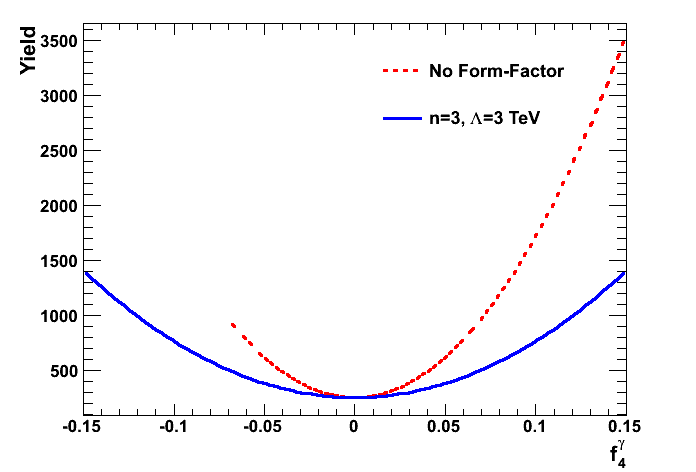
\includegraphics[width=0.47\textwidth]{YieldCoeffs/YieldCoeff_f_4gamma}}
\subfigure[\ffourZ]{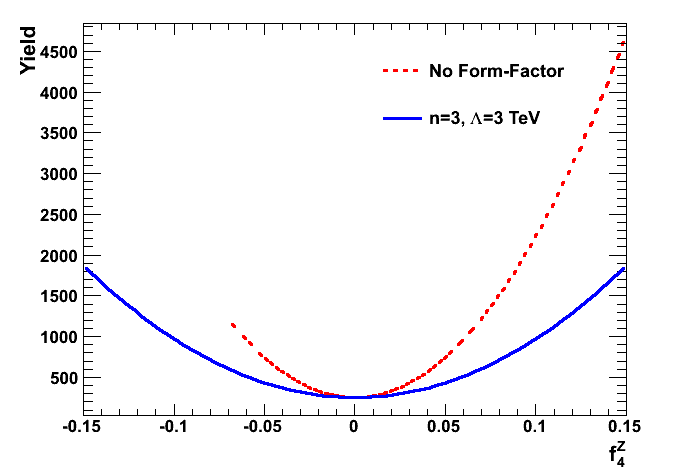
\includegraphics[width=0.47\textwidth]{YieldCoeffs/YieldCoeff_f_4Z}}
\subfigure[\ffiveg]{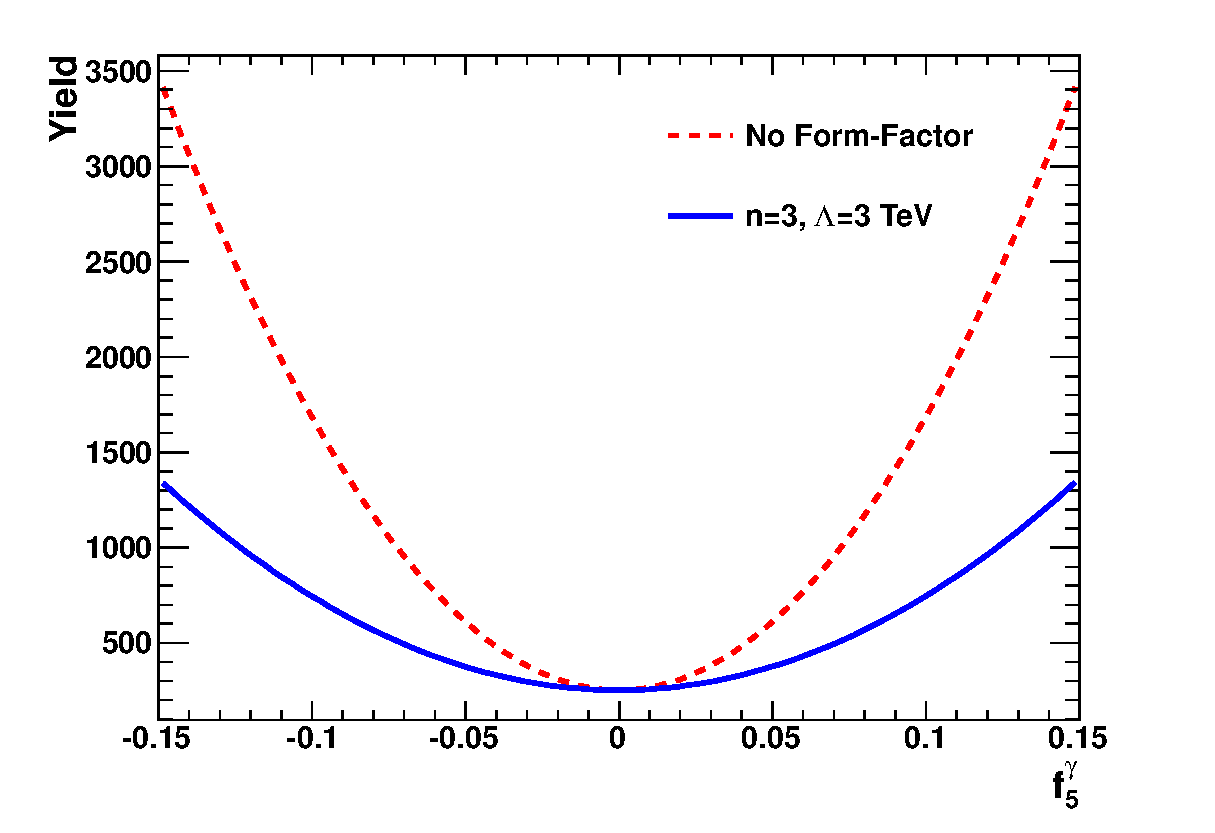
\includegraphics[width=0.47\textwidth]{YieldCoeffs/YieldCoeff_f_5gamma}}
\subfigure[\ffiveZ]{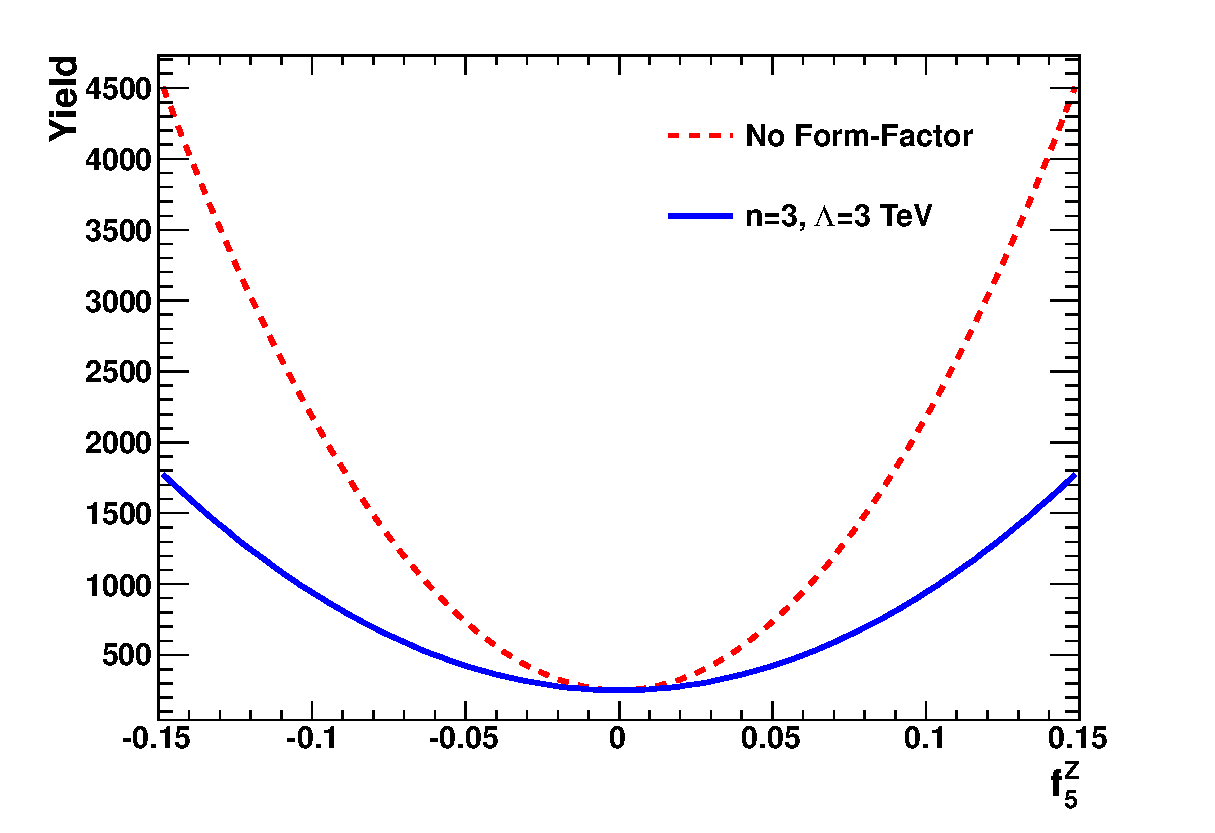
\includegraphics[width=0.47\textwidth]{YieldCoeffs/YieldCoeff_f_5Z}}
\caption{
\small
Expected total event yield for the 8~\tev\ analysis as a function of the \TGC\
parameters: (a) \ffourg, (b) \ffourZ, (c) \ffiveg\ and (d) \ffiveZ. In each
case, the parameters not being varied are assumed to be at their \sm\ values of
zero. The solid blue shows the yields with a \formfactor\ of $n=3,
\Lambda=3~\tev$; the dashed red curve shows the yields with no \formfactor.
 }
\label{fig:TGC-yield-curves}
\end{center}
\end{figure}


\subsection{Limit Setting}
\label{sec:TGC-LimitSetting}

%on the number of observed events in each bin
%of the differential distributions, with systematic uncertainties introduced as
%nuisance parameters. 
95\% confidence level (CL) intervals for the \TGC\ parameters are determined
using a frequentist maximum profile-likelihood based method~\cite{Cowan:2010js},
combining the three \lllplp\ final states prior to
the profile-likelihood maximisation. The likelihood function is similar
to that used in the \cx\ calculation, but parametrised in terms of the
number of events in each bin instead of the \cx. Systematic uncertainties are
again introduced as nuisance parameters 
represented as Gaussian terms ($G$); since there are nuisance
parameters for both signal and background, the set of nuisance parameters giving
the fractional uncertainty on the signal and background expectation for a
distribution of $m$ bins is expressed as:
$\vec\beta = \{\beta_1, \beta_2, \ldots, \beta_{2m}\}$, where:
\begin{eqnarray}
\text{true }N_\mathrm{sig}^i &=& N_\mathrm{sig}^i \cdot (1 + \beta_i) \label{nuis1}\\
\text{true }N_\mathrm{bkg}^i &=& N_\mathrm{bkg}^i \cdot (1 + \beta_{i+m}) \label{nuis2}
\end{eqnarray}
The systematics associated with the theoretical calculation of the fiducial \cx\ in each bin
(due to PDF and scale uncertainties) are assumed to be 100\% correlated between
bins, as are systematic uncertainties on the data-driven background estimate.
Bin by bin correlations of systematics on the expected yield due to
reconstruction uncertainties are propagated for each source of uncertainty via the
covariance matrix. 

The likelihood function is:
\begin{equation}
L(\vec{f}, \vec{\beta}) =
\prod_{i=1}^{m}P(N_\mathrm{obs}^i,\mu^i(\vec{f},\vec\beta))
\times
\frac{1}{(2\pi)^m}e^{-\frac{1}{2}\left(\vec\beta\cdot C^{-1}\cdot\vec\beta\right)},
\label{likelihood}
\end{equation}
where $\vec{f}=\{\ffourg, \ffourZ, \ffiveg, \ffiveZ \}$ are the \TGC\
parameters, $C$ is the covariance matrix, and $\mu^{i}$ is the expected number of events in bin $i$:
\begin{equation}
\mu^i(\vec{f},\vec{\beta})
= N_\mathrm{sig}^i(\vec{f})(1 + \beta_i) + N_\mathrm{bkg}^i(1 + \beta_{i+m}).
\end{equation}
with:
\begin{equation}
N_{\rm sig}(\vec{f}) = \left( Y_\mathrm{\rm SM} + \sum_{i,V} (Y_{f_i^V}\cdot
f_i^V + Y_{f_i^Vf_i^V}\cdot (f_i^V)^2 ) \right) \cdot\mathcal{L}\cdot{C_{ZZ}}.
\end{equation}

A test statistic \teststat\ is constructed as the ratio of the \maxprofilellh\
at a specific test value of the \TGC\ parameters $\vec{f}$ to the full \maxprofilellh:
\begin{equation}
\teststat =
\frac{L(N|\vec{f},\vec{\hat{\hat{\beta}}})}{L(N|\vec{\hat{f}},\vec{\hat{\beta}})}
\end{equation}
where $\vec{\betahathat}$ is the value of $\vec{\beta}$ that maximises the
numerator, and $\vec{\hat{f}}$ and $\vec{\hat{\beta}}$ are the values of
$\vec{f}$ and $\vec{\beta}$ that maximise the numerator. The distribution of
\teststat\ in the assumption of \TGC s at the test value of $\vec{f}$
is obtained by generating 10,000 pseudo experiments. In each
pseudo experiment, the nuisance parameters $\vec{\beta}$ are Gaussian
fluctuated around the mean value of $\vec{\betahathat}$ and the `observed' number of events
is drawn randomly from a Poisson distribution with a mean corresponding to the
values of $\vec{f}$ and $\vec{\beta}$. The $p$-value at the test value of the
couplings is calculated as the fraction of pseudo-experiments which have a test
statistic smaller than the observed value of the test statistic $\teststat_{obs}$.
This procedure is repeated scanning possible values of $\vec{f}$. The 95\%
confidence interval is defined by all values of $\vec{f}$ for which
$p(\vec{f})\geq 5\%$. 

Limits are set for one parameter at a time, holding the other parameters at
their \sm\ values of zero. The expected sensitivity is also obtained using
pseudo-experiments. In each pseudo-experiment, $N^{i}_{sig}$ and $N^{i}_{bg}$
are given by the \sm\ expectations but allowed to fluctuate within their
uncertainties.

\section{Bin Optimisation}
\label{sec:TGC-BinOpt}

For the 7~\tev\ analysis, limits were set using the total number of observed
events, and by using the number of events observed in bins of the leading \Z\
boson candidate \pt\ and in bins of the mass of the four-lepton system. It was found that
binning in the leading \Z\ boson \pt\ yielded the most stringent expected limits, and
that the tightest expected limits were obtained using four bins of \pt\ with boundaries 0-60,
60-100, 100-200 and $>$ 200~\GeV. A combined fit with the results of a \ZZllvv\
analysis was also carried out, using three bins of the leptonically decaying \Z\
candidate for the \ZZllvv\ events.

For the 8~\tev\ analysis, a bin optimisation was carried out, varying
the number of bins and the bin boundaries. For each variation, a set of 5,000
pseudo-experiments is carried out in order to derive the expected limit. The systematic uncertainties on the expected signal
in each bin are re-evaluated, as well the theoretical uncertainties on the
differential \cx. The estimated irreducible background is re-derived from the
\mc. An estimated for the reducible background in each bin is obtained by dividing the total
data-driven reducible background estimate according to the background shape obtained from data. The
fractional systematic and statistical uncertainties on the data-driven background
estimate are assumed to be the same in every bin. No systematic to
account for uncertainties on the reducible background shape is assigned. This
approximation is justified by the fact that the total background uncertainty is
already large, and that the background contribution when the leading \Z\ has
\pt\ above 100~\gev\ is very small.
This procedure means that large statistical and systematic uncertainties on the
expected signal and large PDF and scale errors on the fiducial \cx\ when the last bin boundary is
very high are taken into account in the expected limits. It does
not, however, take into account the fact that there may be insufficient \mc\
statistics associated with the estimate of the reconstruction systematic uncertainties when
there are limited statistics in the \sm\ \mc\ sample in the last bin. Therefore
before choosing a final binning it is checked that the statistics in the last
bin are sufficient to properly evaluate the systematics.

A variety of choices of binning were tried, varying the number of bins from one
to five, and varying the boundaries of the bins. It is observed that the
observed limits are most sensitive to the lower boundary of the last bin, which
is taken to be inclusive (i.e. including all events with \Z\ boson \pt\ greater
than the lower bin boundary). The limits are observed not to be very sensitive
to the number of bins or the boundaries of the bins other than the last.
\fig{TGC-binOpt} shows the expected limit on \ffourg\ as a function of the lower
boundary of the last bin. Limits obtained using different numbers of bins are
shown as different coloured markers. The expected limits become more stringent
as the lower boundary of the last bin increases, but varying the bin boundaries
other than the lower boundary of the last bin has little effect on the expected
limits.  The tightening of the limits as the boundary of the last bin is
increased is because the relative increase in signal yield due to the existence
of \TGC s is much larger at higher \Z\ boson \pt. It is seen that beyond
300~\gev\ the limits do not significantly improve, since past this point the
signal expectation in the case of \sm\ couplings only becomes very small, and so
increasing the bin boundary further does little to increase the significance of
the \TGC\ signal. Beyond 550~\gev, the expected limits worsen; this is because
the statistical, systematic, and theoretical uncertainties on the expected
signal become very large, as can be seen in~\fig{TGC-uncertainties} which shows
the percentage uncertainty due to the signal and background statistical and
systematic uncertainties, and from theoretical uncertainties on the fiducial
\cx, for a variety of choices of binning.
%Full details of the different bin boundaries tried
%are given in~\app{}.

\begin{figure}[htbp]
\begin{center}
\subfigure[]{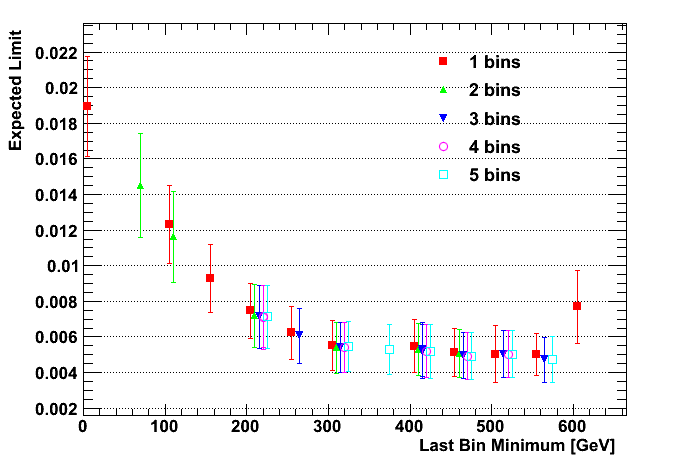
\includegraphics[width=0.7\textwidth]{BinOpt/BinOpt_BinOpt_02_130325_newSyst_f4g}}
\caption{
\small
Expected limits on \ffourg\ obtained in a binned fit of the \pt\ distribution of
the leading \Z\ boson candidate, as a function of the lower boundary of the last bin
in \pt. The different coloured markers show the limits obtained using 
different numbers of bins.
 }
\label{fig:TGC-binOpt}
\end{center}
\end{figure}

\begin{figure}[htbp]
\begin{center}
\subfigure[0-300, $>$300~\gev]{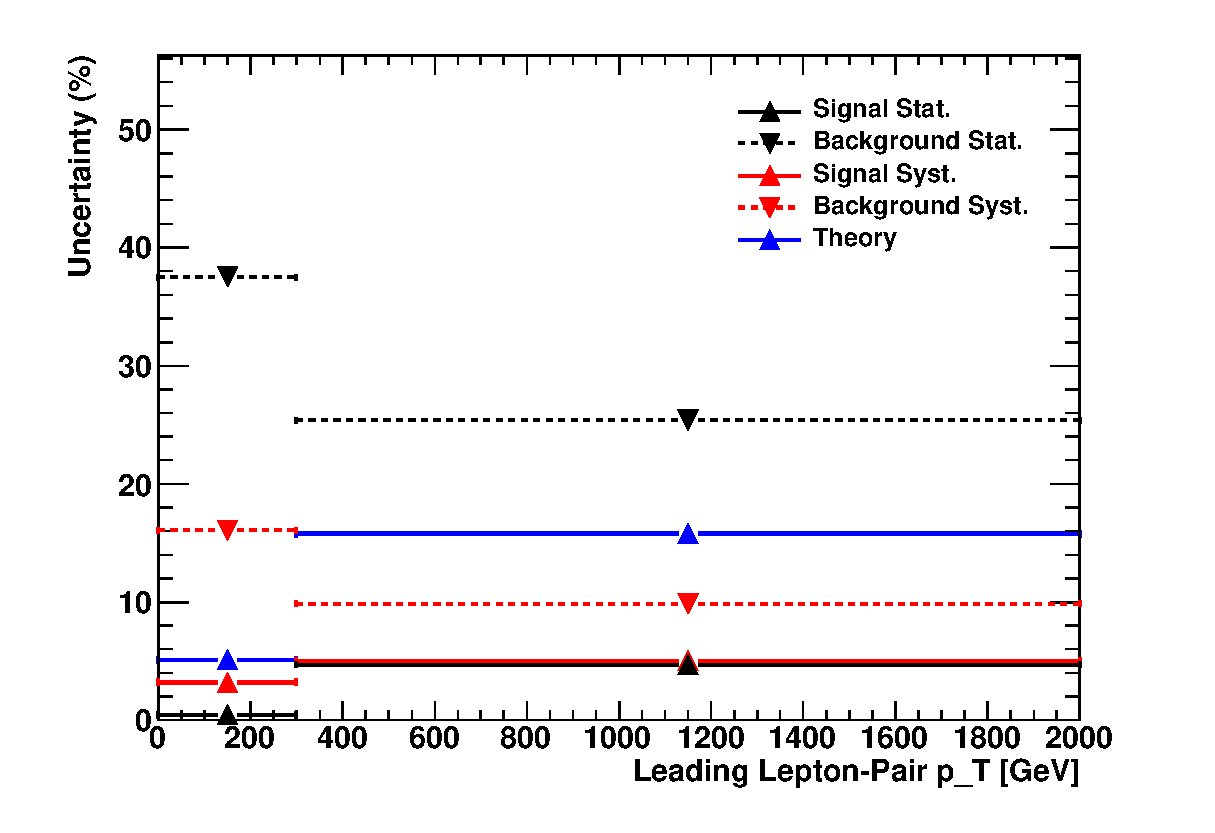
\includegraphics[width=0.47\textwidth]{{BinOpt/PtZ1_2Bin_3_TGCLimInput._UncertaintiesPlot}.eps}}
\subfigure[0-500, $>$500~\gev]{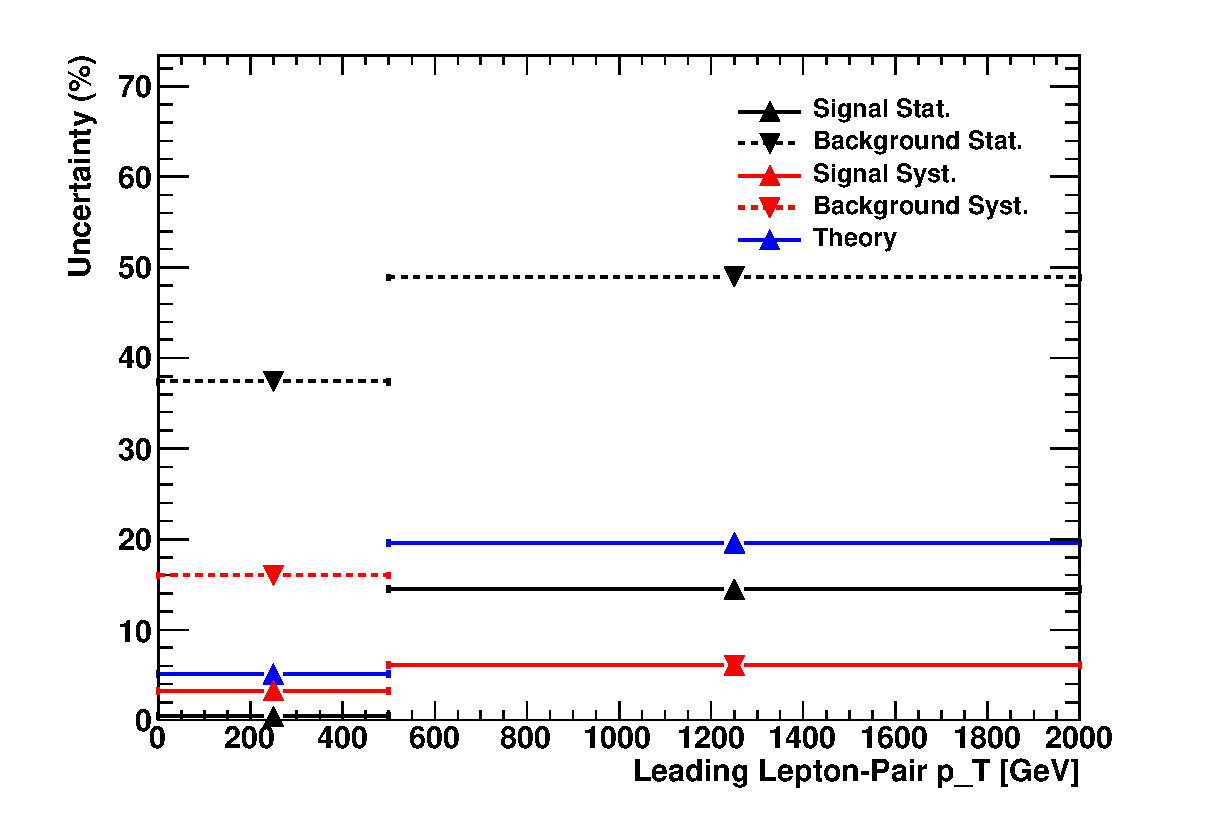
\includegraphics[width=0.47\textwidth]{{BinOpt/PtZ1_2Bin_6_TGCLimInput._UncertaintiesPlot}.eps}}
\subfigure[0-600, $>$600~\gev]{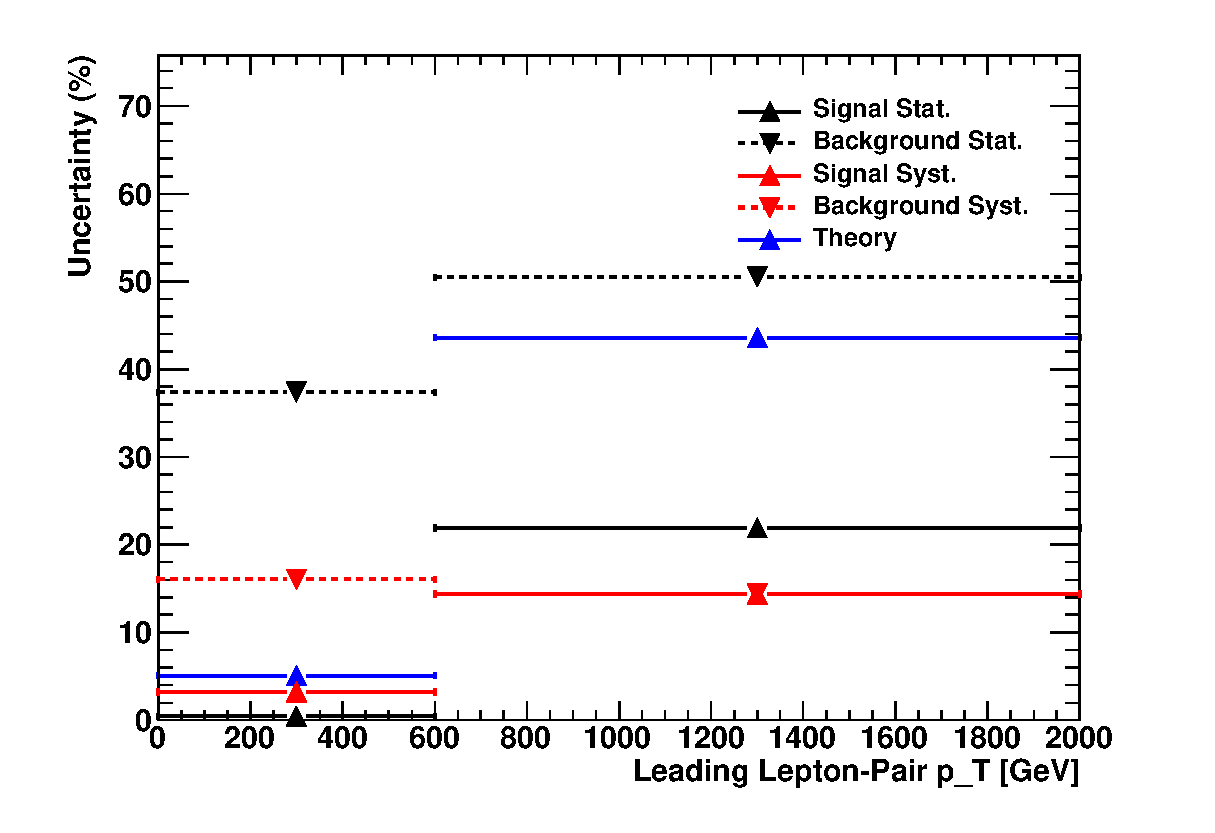
\includegraphics[width=0.47\textwidth]{{BinOpt/PtZ1_2Bin_13_TGCLimInput._UncertaintiesPlot}.eps}}
\caption{
\small
Percentage uncertainties from for different choices of binning
in the \pt\ of the leading \Z\ boson. The black upwards triangles show the
statistical uncertainty on the signal expectation and the black downwards
triangles the statistical uncertainty on the background estimate. The red
upwards triangle show the systematic uncertainty on the signal expectation and
the red downwards triangles the systematic uncertainty on the background. The
blue upwards triangles show the theoretical uncertainty on the signal
expectation.
 }
\label{fig:TGC-uncertainties}
\end{center}
\end{figure}

The final limits are set using two bins of leading \Z\ boson \pt: 0-300 and $>$
300~\gev. This binning was chosen as it gives similar limits to choices of
binning where the last bin boundary is higher in \pt, but retains sufficient
statistics in the signal \mc\ in order to estimate the systematic uncertainties.
Increasing the number of bins was not seen to give any improvement in the
expected limits, so for computational convenience the binning with the lowest
number of bins was chosen.

\section{Robustness of Limits}
\label{sec:TGC-Robustness}

In order to check the robustness of the limits, the expected limits obtained
using the \BR\ matrix-elements to determine the yield coefficients are compared with
the expected limits obtained using \BHO\ matrix-elements to determine to coefficients.
Similarly, the expected limits obtained using a samples samples generated at
different TGC points are compared (e.g. the TGC0 sample is compared to the TGC1
sample). Full details of the comparison are given
in~\app{TGC-Robustness}; the changes in expected limits are much smaller
than the statistical uncertainties on the limit.

In order to check the effect of the assumption that the fractional statistical and
systematic uncertainties on the
data-driven reducible background estimate are the same in each bin of the leading \Z\
boson \pt, expected limits are obtained with the data-driven background
uncertainties increased by a factor of five. The resulting changes in the
expected limits are less than 1\%, justifying this assumption.

\section{Expected and Observed Limits}
\label{sec:TGC-ExpObsLimits}

\fig{tgc-nicePlot} shows observed and expected distributions of the \pt\ of
leading \Z\ candidate with the binning used to set the limits, along with
expected distributions for \TGC\ values set close to the previously obtained
limits.

% Expected Observed with TGC binning
\begin{figure}[htbp]
\begin{center}
\subfigure[] {
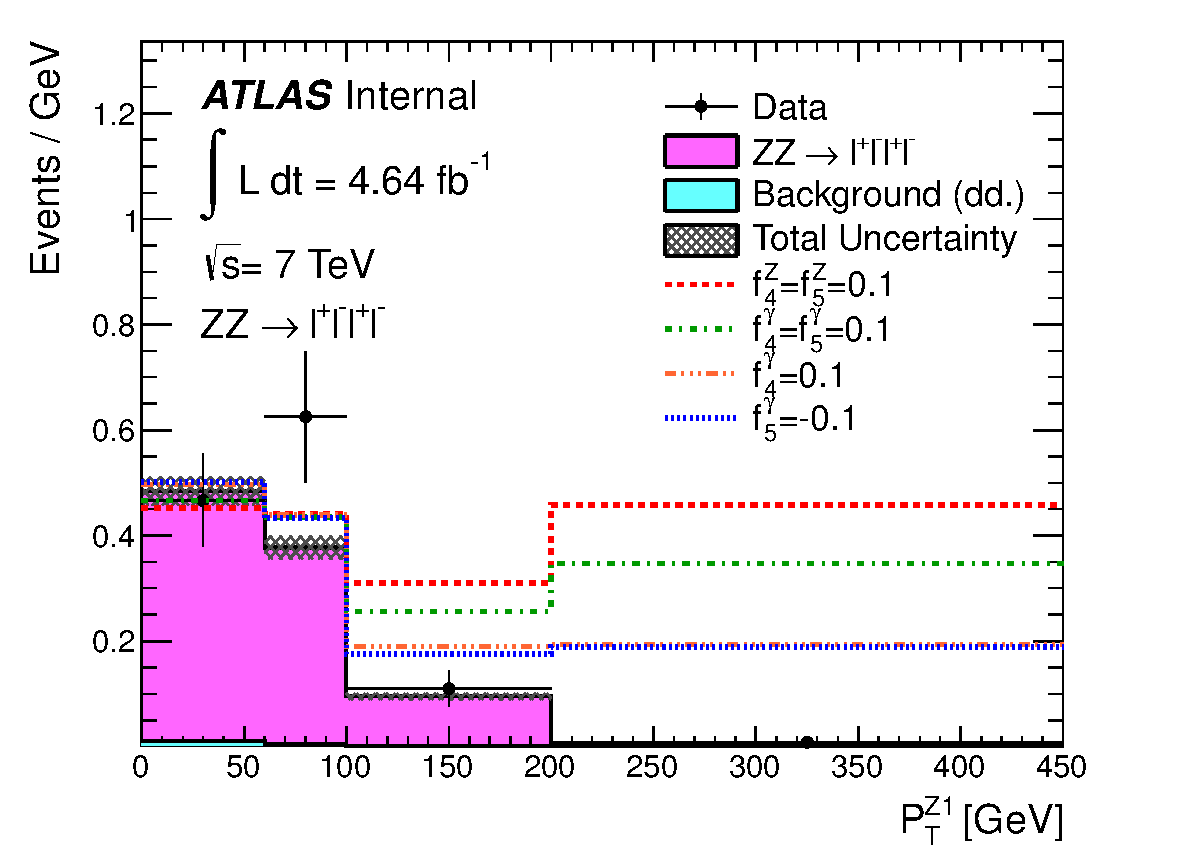
\includegraphics[width=0.47\textwidth]{NicePlots/h_4l_ZZ_Z1_pt_withTGC_Lambda3TeV}
}
\subfigure[] {
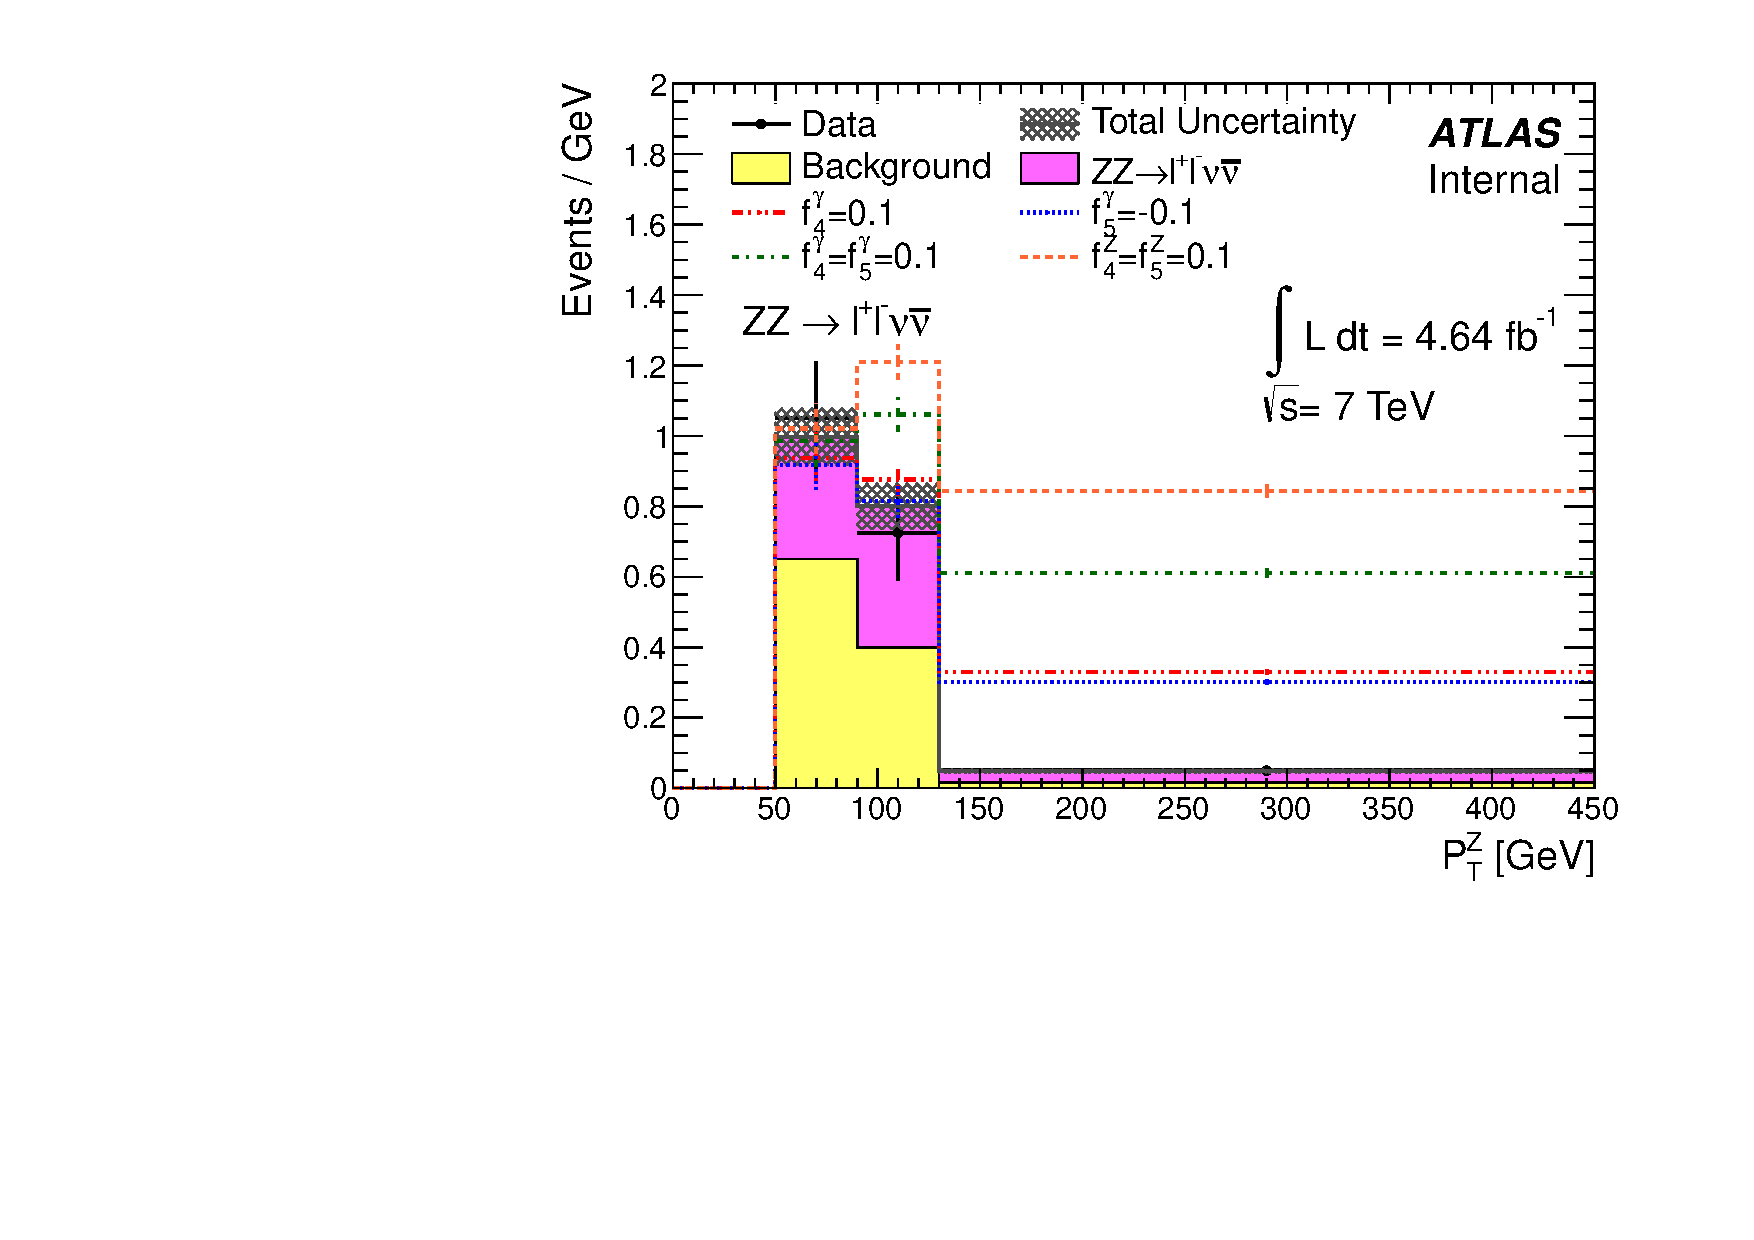
\includegraphics[width=0.47\textwidth]{NicePlots/h_2l2n_ZZ_Z1_pt_withTGC_Lambda3TeV}
}
\subfigure[] {
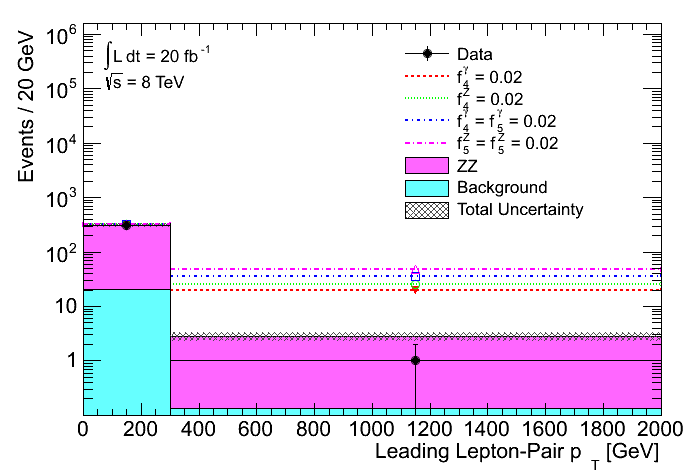
\includegraphics[width=0.47\textwidth]{NicePlots/FinalBinning_01_130326_PtZ1_2Bin_3_BR_n3L3_NicePlot}
}
\caption[\Z-boson transverse momentum distributions with the binning used for
TGC limit setting.]
{\Z-boson transverse momentum distributions with the binning used for
TGC limit setting.
Figure (a) shows the $p_T$ of the leading \Z\ candidate for the \ZZllll\ channel and (b) shows
the $p_T$ of the leptonically decaying \Z\ candidate for the \ZZllvv\ channel, both in the
7~\tev\ data. Figure (c) shows the \pt\ of the leading \Z\ candidate for the \ZZllll\ channel
for the 8~\tev\ data.
The observed distributions are shown as filled circles,
the SM expected signal and background are shown as filled histograms, and the
predicted distributions for four different \TGC\ samples with form factor
 scales of $\Lambda=3$ TeV are shown as dashed lines.
The \TGC\ parameters in Figures (a) and (b) are 
 set near the edge of the exclusion set in the 1 fb$^{-1}$
 analysis~\cite{ATLAS_ZZ4l:1fb2011}; the \TGC parameters in Figure (c) are
 set near the limits obtained from the 7~\tev\ analysis.}
\label{fig:tgc-nicePlot}
\end{center}
\end{figure}

% \begin{landscape}
% \thispagestyle{lscape}
%\begin{table}[htbp]
%\centering
%\small
%\begin{tabular}{lcccc}
%\hline\hline
%No. Bins& \ffourg\ & \ffourZ\ & \ffiveg\ & \ffiveg \\
%\hline
%\multicolumn{2}{l}{\underline{\bf $n=3, \Lambda=3~\tev$} } \\
%      1  &  [-0.032, 0.032 ] $\pm$ 0.005 &  [-0.027, 0.027 ] $\pm$ 0.004 &  [-0.033, 0.033 ] $\pm$ 0.005 &  [-0.028, 0.028 ] $\pm$ 0.004 \\
%      2  &  [-0.010, 0.010 ] $\pm$ 0.003 &  [-0.009, 0.009 ] $\pm$ 0.002 &  [-0.010, 0.010 ] $\pm$ 0.003 &  [-0.009, 0.009 ] $\pm$ 0.002 \\
%\hline
%\multicolumn{2}{l}{\underline{ No Form Factor} } \\
%      1  &  [-0.019, 0.019 ] $\pm$ 0.003 &  [-0.016, 0.016 ] $\pm$ 0.002 &  [-0.019, 0.019 ] $\pm$ 0.003 &  [-0.016, 0.017 ] $\pm$ 0.002 \\
%      2  &  [-0.005, 0.005 ] $\pm$ 0.001 &  [-0.005, 0.005 ] $\pm$ 0.001 &  [-0.005, 0.005 ] $\pm$ 0.001 &  [-0.005, 0.005 ] $\pm$ 0.001 \\
%\hline\hline
%\end{tabular}
%\end{table}
%\end{landscape}

\begin{table}[htbp]
\centering
\small
\begin{tabular}{lcccc}
\hline\hline
Parameter & Expected Limit                & Observed Limit \\
\hline
\multicolumn{2}{l}{\underline{$n=3, \Lambda=3~\tev$, \ZZllll } } \\
\ffourg   &  [-0.027, 0.027 ] $\pm$ 0.007 & [-0.031, 0.031 ] \\
\ffourZ   &  [-0.023, 0.023 ] $\pm$ 0.006 & [-0.027, 0.027 ] \\
\ffiveg   &  [-0.028, 0.028 ] $\pm$ 0.007 & [-0.032, 0.032 ] \\
\ffiveZ   &  [-0.023, 0.023 ] $\pm$ 0.006 & [-0.027, 0.027 ] \\
\hline                                                       
\multicolumn{2}{l}{\underline{$n=3, \Lambda=3~\tev$, \ZZllllorvv} } \\
\ffourg   &  [-0.021, 0.022 ] $\pm$ 0.003 & [-0.022, 0.023 ] \\
\ffourZ   &  [-0.017, 0.018 ] $\pm$ 0.003 & [-0.019, 0.019 ] \\
\ffiveg   &  [-0.022, 0.022 ] $\pm$ 0.004 & [-0.023, 0.023 ] \\
\ffiveZ   &  [-0.018, 0.018 ] $\pm$ 0.003 & [-0.020, 0.019 ] \\
\hline
\multicolumn{2}{l}{\underline{No Form Factor, \ZZllll} } \\
\ffourg   &  [-0.017, 0.017 ] $\pm$ 0.004 & [-0.020, 0.020 ] \\
\ffourZ   &  [-0.015, 0.015 ] $\pm$ 0.002 & [-0.017, 0.017 ] \\
\ffiveg   &  [-0.018, 0.018 ] $\pm$ 0.004 & [-0.020, 0.020 ] \\
\ffiveZ   &  [-0.015, 0.015 ] $\pm$ 0.004 & [-0.017, 0.017 ] \\
\hline                                                                          
\multicolumn{2}{l}{\underline{No Form Factor, \ZZllllorvv} } \\
\ffourg   &  [-0.014, 0.014 ] $\pm$ 0.001 & [-0.015, 0.015 ] \\
\ffourZ   &  [-0.012, 0.012 ] $\pm$ 0.001 & [-0.013, 0.013 ] \\
\ffiveg   &  [-0.015, 0.015 ] $\pm$ 0.001 & [-0.016, 0.015 ] \\
\ffiveZ   &  [-0.012, 0.012 ] $\pm$ 0.001 & [-0.013, 0.013 ] \\
\hline\hline
\end{tabular}
           \caption{
           Expected and observed 95\% confidence intervals for anomalous neutral
           gauge boson couplings (\TGC s), set using the 7~\tev\ data, where 
           the limit for each coupling assumes the other couplings
           fixed at their SM value of zero. 
           Limits are given for \formfactor\ scales of $\Lambda = 3$ \TeV\
           and $\Lambda = \infty$, the latter corresponding to not applying a \formfactor. 
           %They include 
           %both statistical and systematic uncertainties; the statistical uncertainties are dominant.
           }
           \label{table:TGC-obs-exp-limits-seven}
\end{table}

\tabs{TGC-obs-exp-limits-seven}{TGC-obs-exp-limits-eight} show the observed and
expected 95\% confidence interval limits obtained using the 7~\tev\ and the
8~\tev\ data, respectively. The limit on each coupling assumes the other
couplings are fixed at their \sm\ value of zero. In both datasets, no evidence
for \TGC s is observed, and the observed limits are consistent with the expected
limits. The expected limits using the 8~\tev\ data are 2.4-3.0 times more
stringent than the expected limits using the 7~\tev\ dataset using both the
\ZZllll\ and \ZZllvv\ channels, or 3.0-3.6 times more stringent than the
expected limits using only the \ZZllll\ channel of the 7~\tev\ data.

\fig{TGC-limits-2D} shows `two-dimensional' 95\%
confidence level limits, allowing two of the couplings to vary simultaneously,
derived without using a \formfactor. The plots compare the limits set
with the 7~\tev\ data using only the \ZZllll\ channel, the limits set with the 7~\tev\ combining the \ZZllll\ and \ZZllvv\
channels, and the limits obtained with the 8~\tev\
data using only the \ZZllll. For each pair of parameters, the other parameters
are assumed to be fixed at their \sm\ value of zero. 

%The horizontal and vertical lines

%correspond to the one dimensional limits.
A comparison of the limits presented here those derived from measurements at
LEP, Tevatron and CMS is shown in~\fig{TGC-SummaryPlot}.  The one-dimensional
limits are more stringent than those derived from measurements at
LEP~\cite{bib:LEPEW2006} and the Tevatron~\cite{Abazov:2007ad} and previously by
ATLAS~\cite{ATLAS_ZZ4l:1fb2011}. The ATLAS \sqrtseq{7} limits are comparable to
the limits from CMS derived at the same centre-of-mass energy using a similarly
sized dataset. It should be noted that the limits from LEP and CMS do not use a
form factor, and those from the Tevatron use $\Lambda = 1.2\TeV$.

\begin{table}[htbp]
\centering
\small
\begin{tabular}{lcccc}
\hline\hline
Parameter & Expected Limit                & Observed Limit \\
\hline
%\multicolumn{2}{l}{\underline{$n=3, \Lambda=3~\tev$, 1 Bin} } \\
%\ffourg   &  [-0.032, 0.032 ] $\pm$ 0.005 & [-0.030, 0.029 ] \\
%\ffourZ   &  [-0.027, 0.027 ] $\pm$ 0.004 & [-0.025, 0.025 ] \\
%\ffiveg   &  [-0.032, 0.033 ] $\pm$ 0.005 & [-0.030, 0.030 ] \\
%\ffiveZ   &  [-0.028, 0.028 ] $\pm$ 0.004 & [-0.025, 0.026 ] \\
%\hline                                                       
\multicolumn{2}{l}{\underline{$n=3, \Lambda=3~\tev$, \ZZllll} } \\
\ffourg   &  [-0.010, 0.010 ] $\pm$ 0.003 & [-0.007, 0.007 ] \\
\ffourZ   &  [-0.008, 0.009 ] $\pm$ 0.002 & [-0.006, 0.006 ] \\
\ffiveg   &  [-0.010, 0.010 ] $\pm$ 0.003 & [-0.007, 0.007 ] \\
\ffiveZ   &  [-0.009, 0.009 ] $\pm$ 0.002 & [-0.006, 0.006 ] \\
\hline
%\multicolumn{2}{l}{\underline{No Form Factor, 1 Bin} } \\
%\ffourg   &  [-0.019, 0.019 ] $\pm$ 0.003 & [-0.017, 0.017 ] \\
%\ffourZ   &  [-0.016, 0.016 ] $\pm$ 0.002 & [-0.015, 0.015 ] \\
%\ffiveg   &  [-0.019, 0.019 ] $\pm$ 0.003 & [-0.018, 0.018 ] \\
%\ffiveZ   &  [-0.016, 0.017 ] $\pm$ 0.002 & [-0.015, 0.015 ] \\
%\hline                                                                          
\multicolumn{2}{l}{\underline{No Form Factor,  \ZZllll }} \\
\ffourg   &  [-0.005, 0.005 ] $\pm$ 0.001 & [-0.004, 0.004 ] \\
\ffourZ   &  [-0.005, 0.005 ] $\pm$ 0.001 & [-0.003, 0.003 ] \\
\ffiveg   &  [-0.005, 0.005 ] $\pm$ 0.001 & [-0.004, 0.004 ] \\
\ffiveZ   &  [-0.005, 0.005 ] $\pm$ 0.001 & [-0.003, 0.003 ] \\
\hline\hline
\end{tabular}
           \caption{
           Expected and observed 95\% confidence intervals for anomalous neutral
           gauge boson couplings (\TGC s), set using the 8~\tev\ data, where 
           the limit for each coupling assumes the other couplings
           fixed at their \sm\ value of zero. 
           Limits are given for \formfactor\ scales of $\Lambda = 3$ \TeV\
           and $\Lambda = \infty$, the latter corresponding to not applying a \formfactor. 
           %They include 
           %both statistical and systematic uncertainties; the statistical uncertainties are dominant.
           }
           \label{table:TGC-obs-exp-limits-eight}
\end{table}

\begin{figure}[htbp]
\begin{center}
\subfigure{
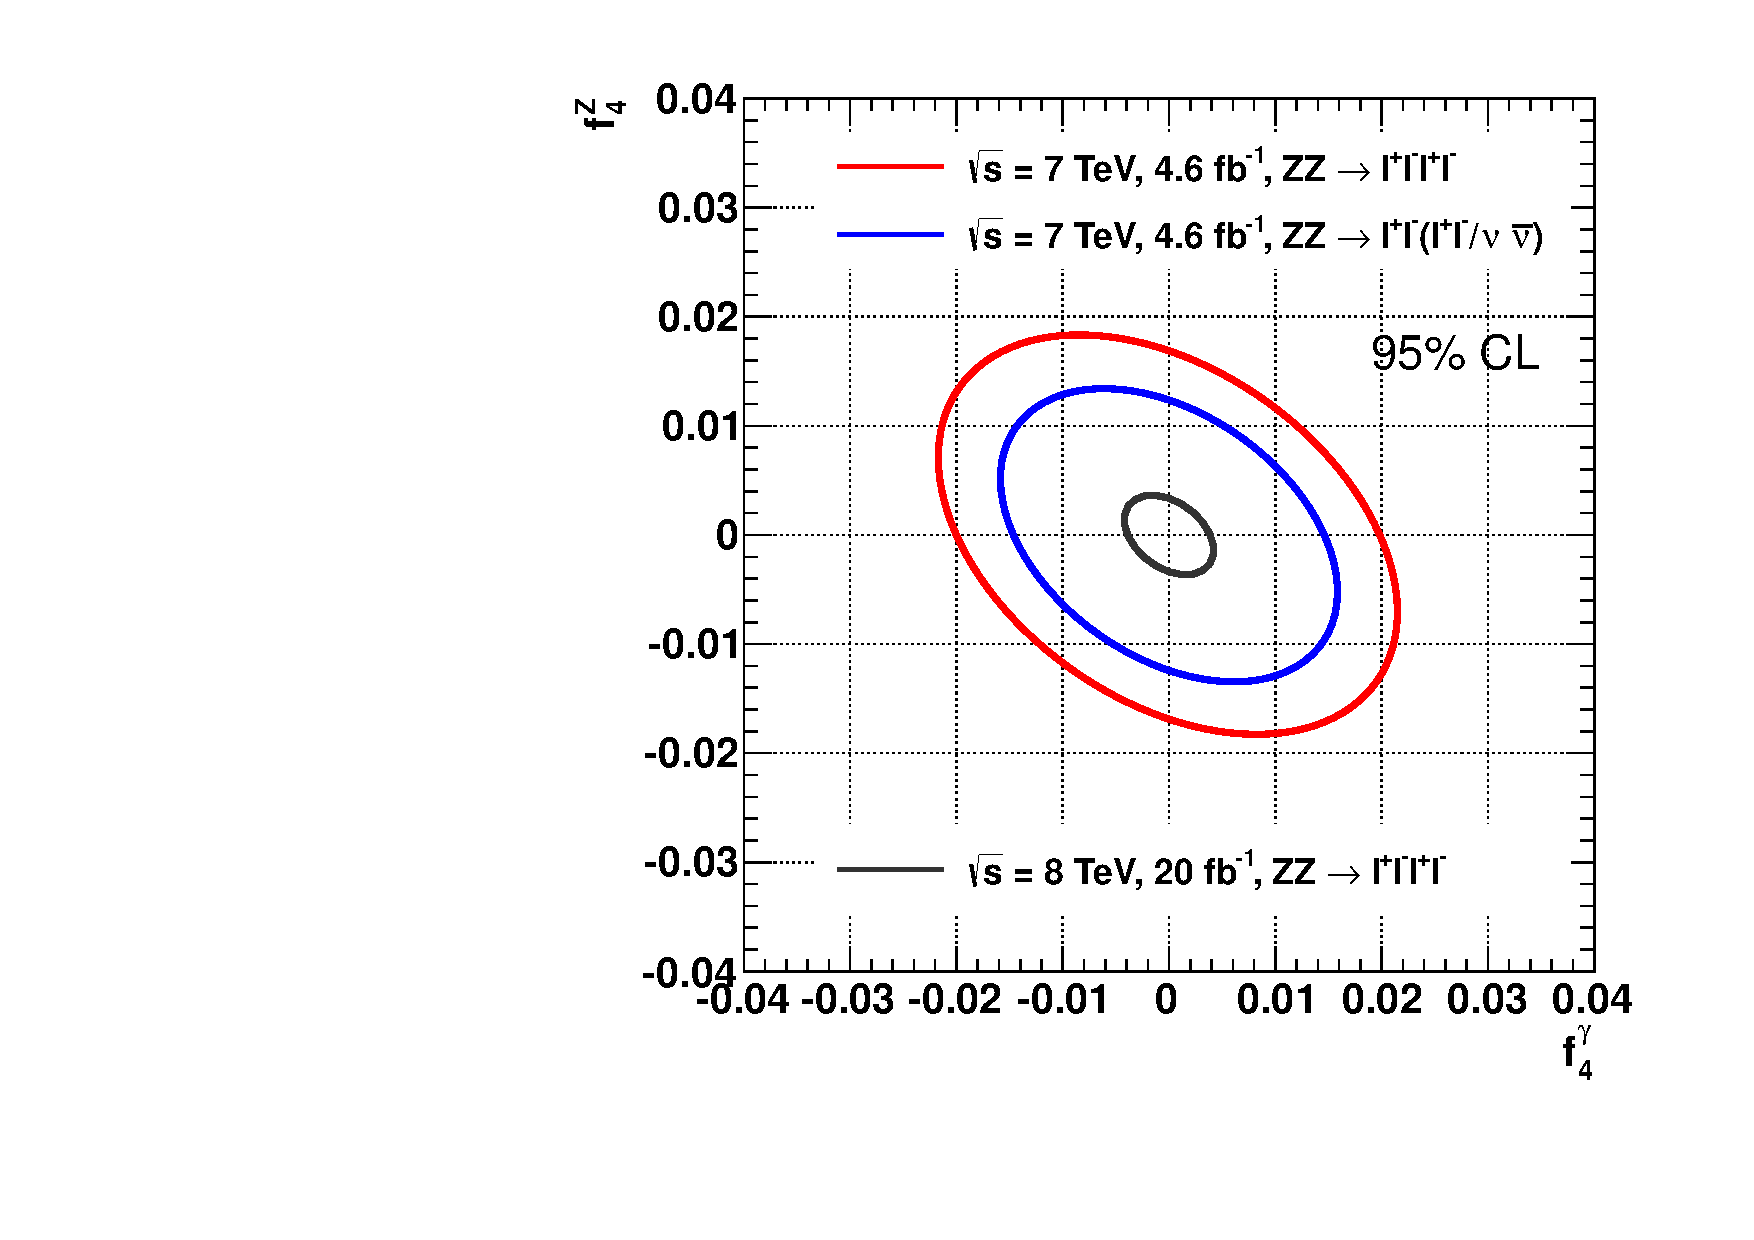
\includegraphics[width=0.43\textwidth]{2D_7TeV_8TeV/frequentist_f4Z_f4g}
}                                                                      
\subfigure{                                                          
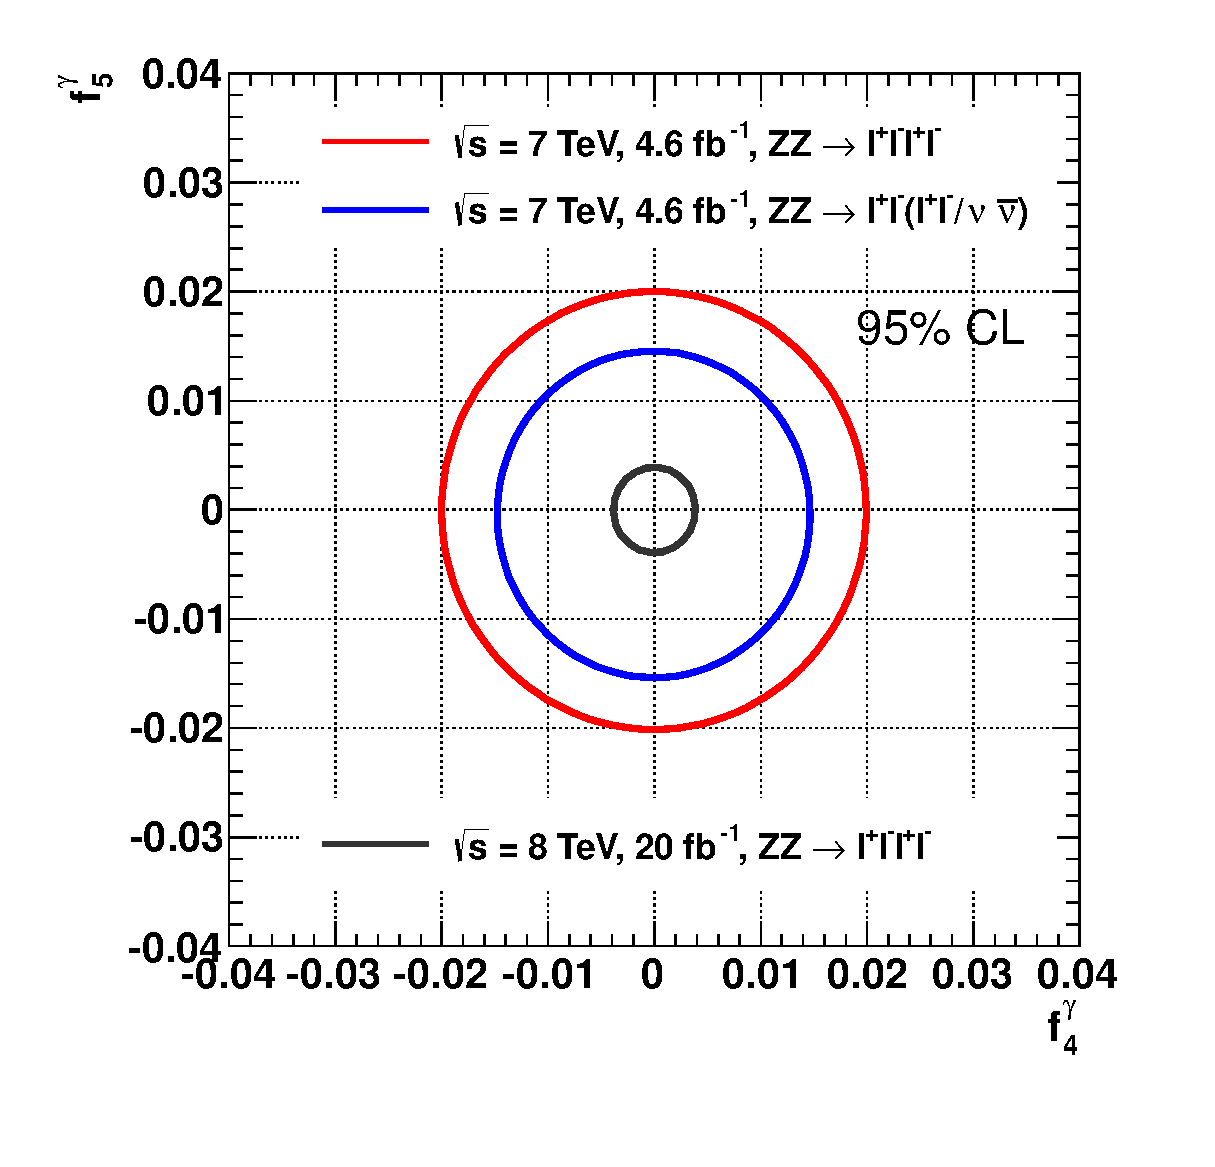
\includegraphics[width=0.43\textwidth]{2D_7TeV_8TeV/frequentist_f5g_f4g}
}                                                                      
\subfigure{                                                          
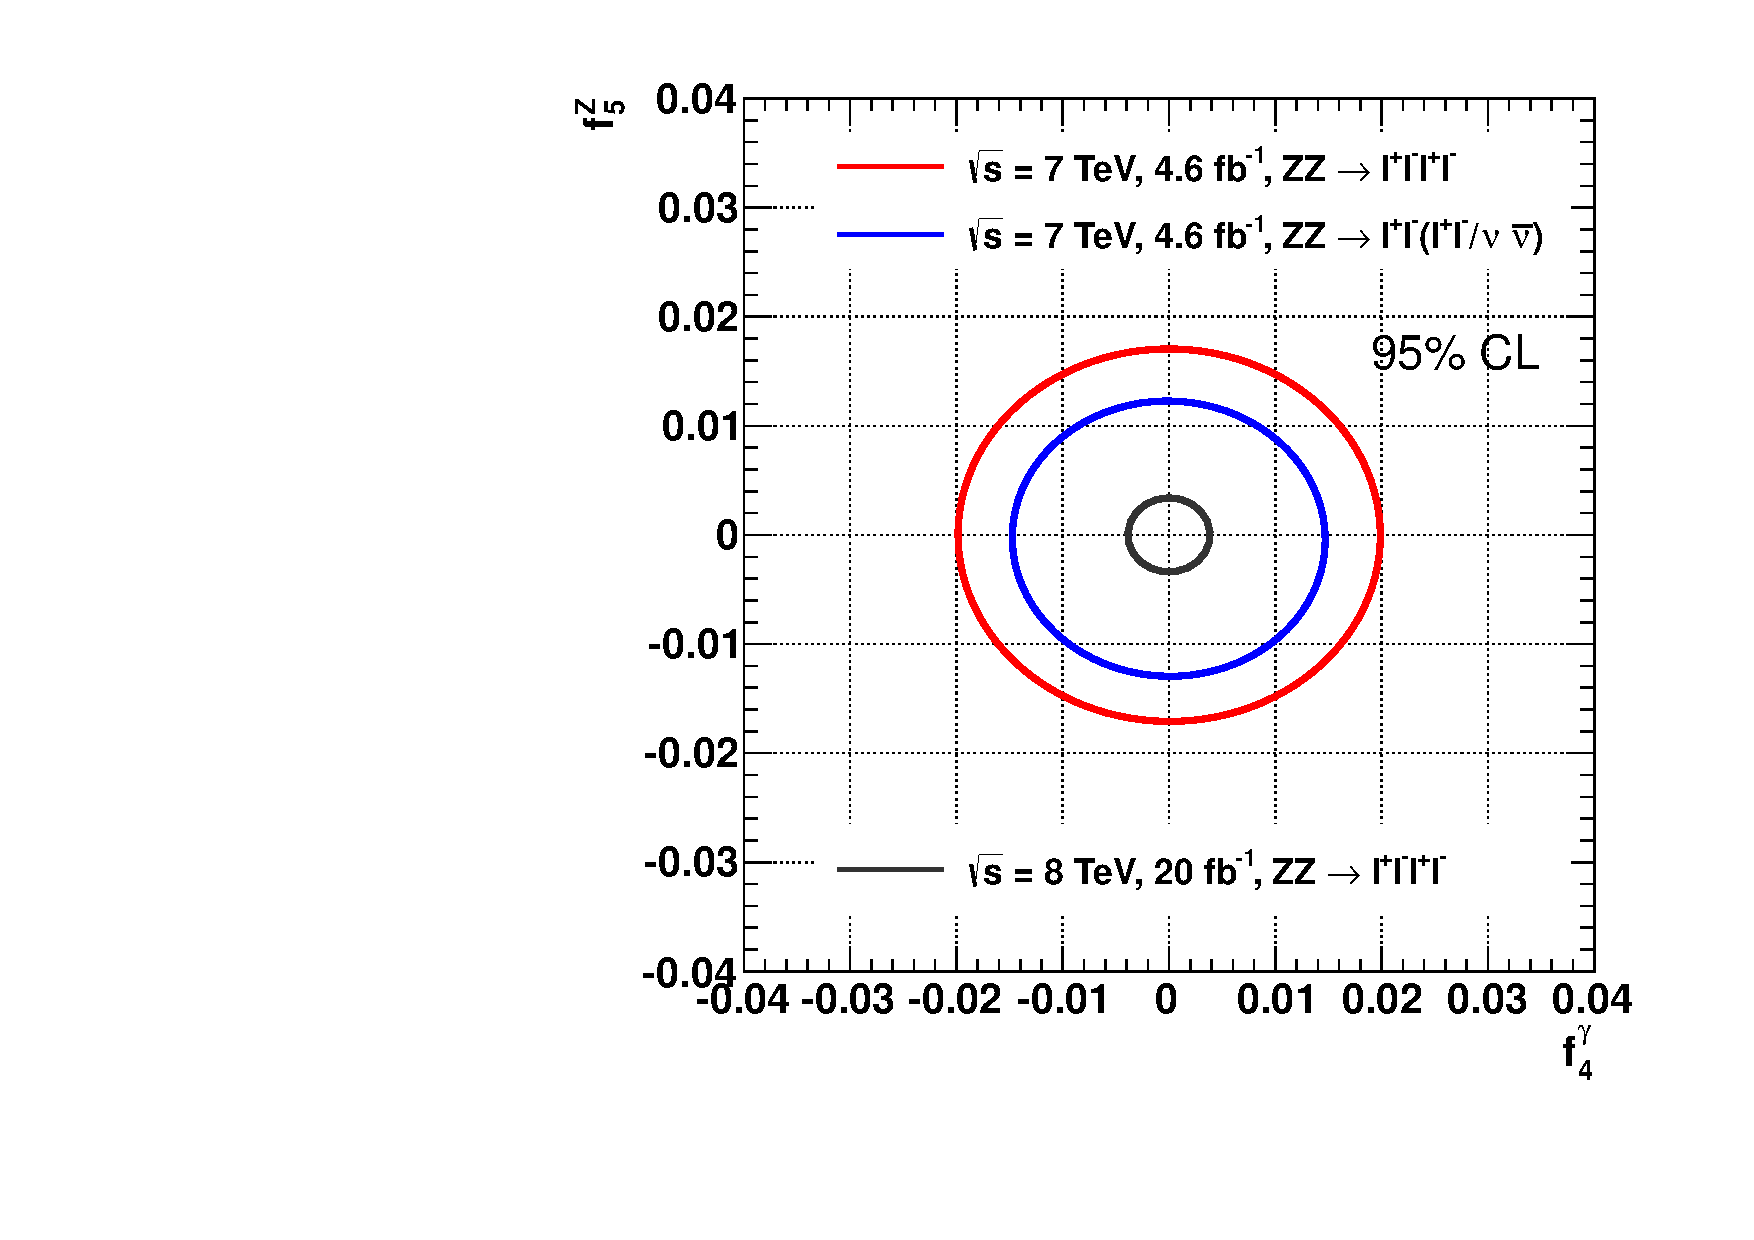
\includegraphics[width=0.43\textwidth]{2D_7TeV_8TeV/frequentist_f5Z_f4g}
}                                                                      
\subfigure{                                                          
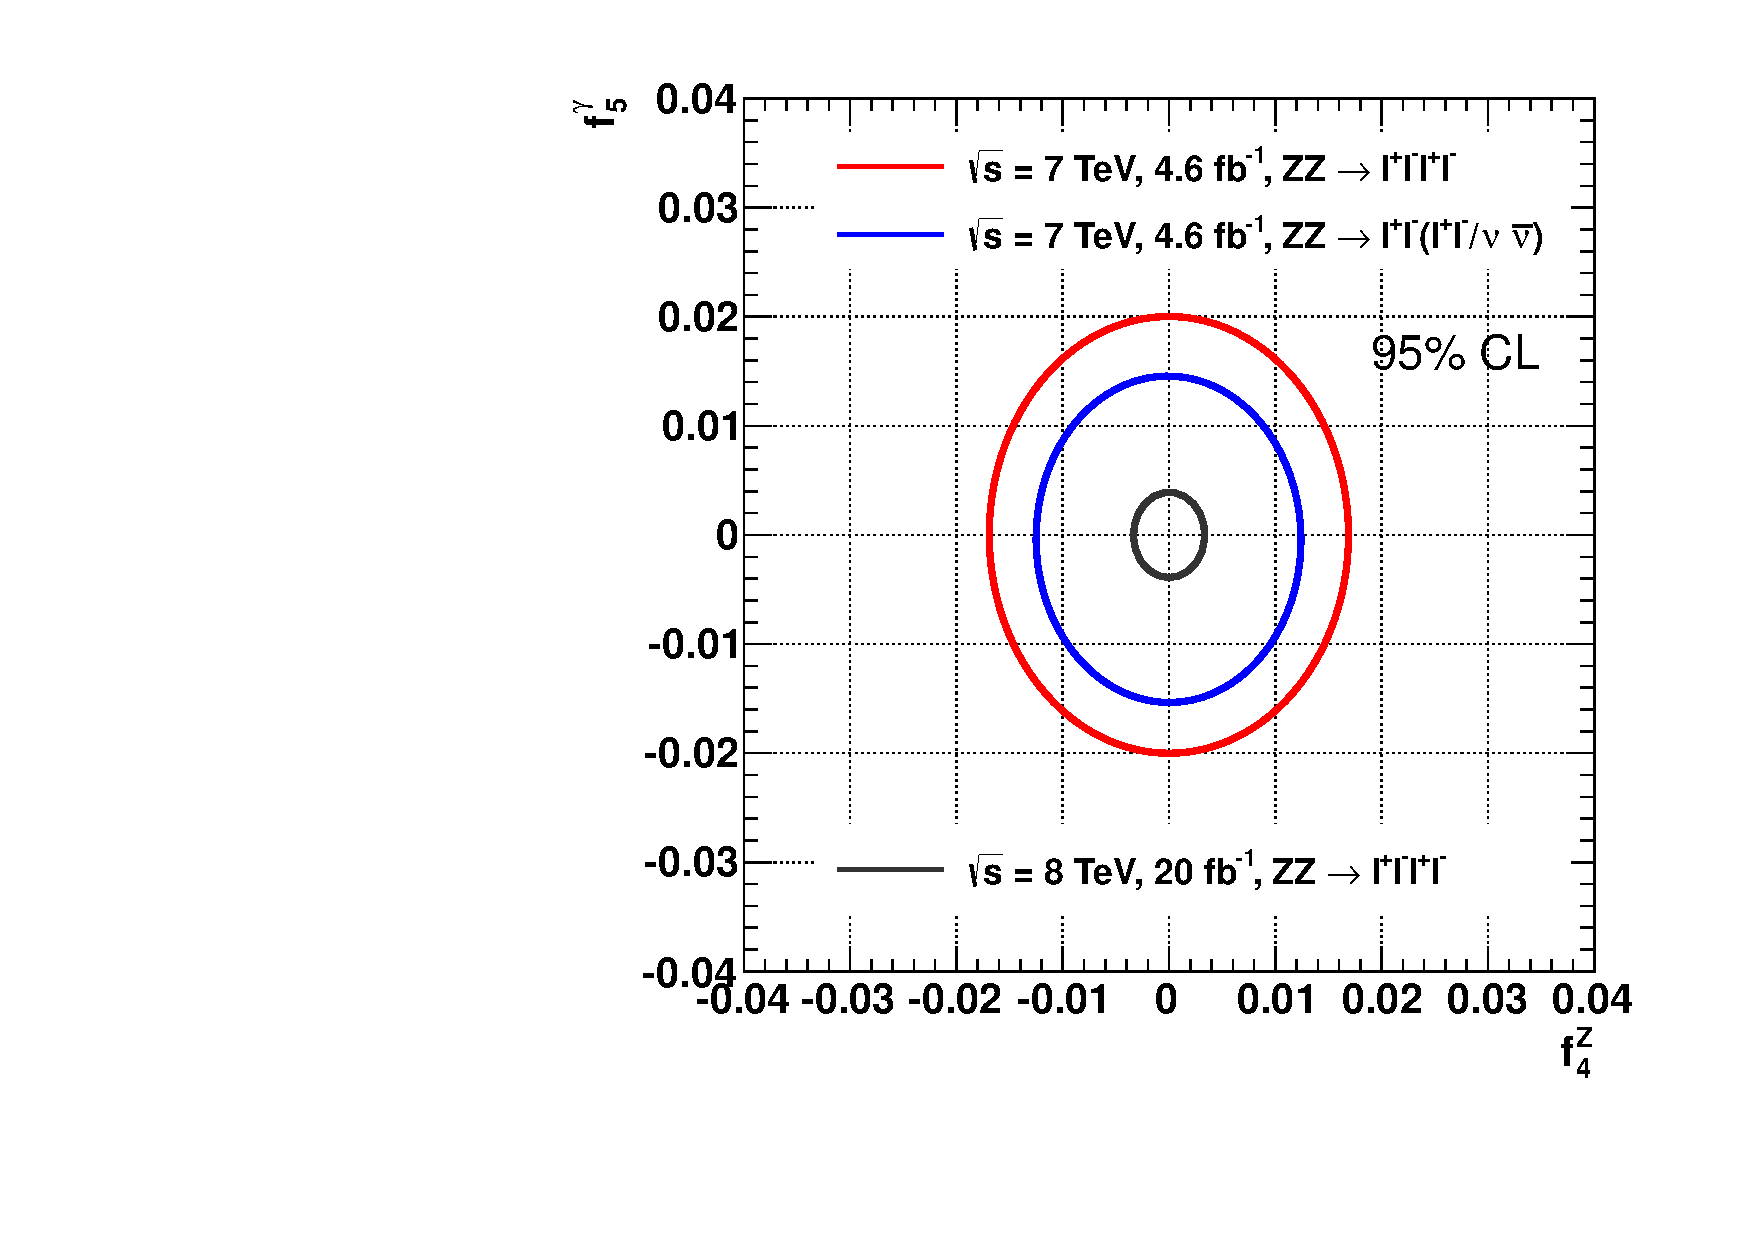
\includegraphics[width=0.43\textwidth]{2D_7TeV_8TeV/frequentist_f5g_f4Z}
}                                                                      
\subfigure{                                                          
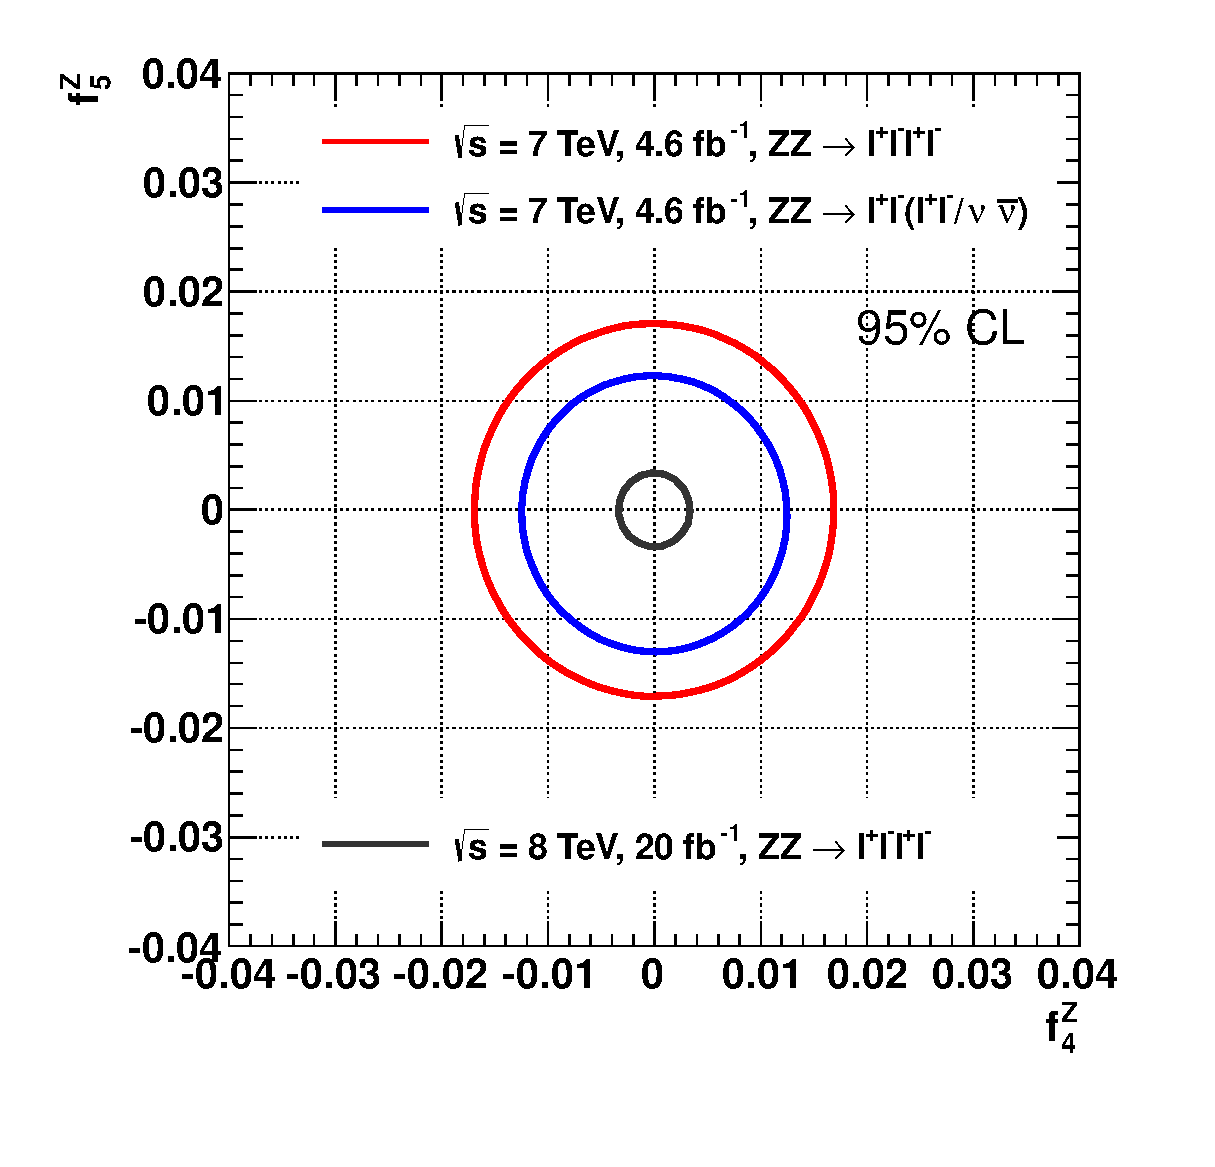
\includegraphics[width=0.43\textwidth]{2D_7TeV_8TeV/frequentist_f5Z_f4Z}
}                                                                      
\subfigure{                                                          
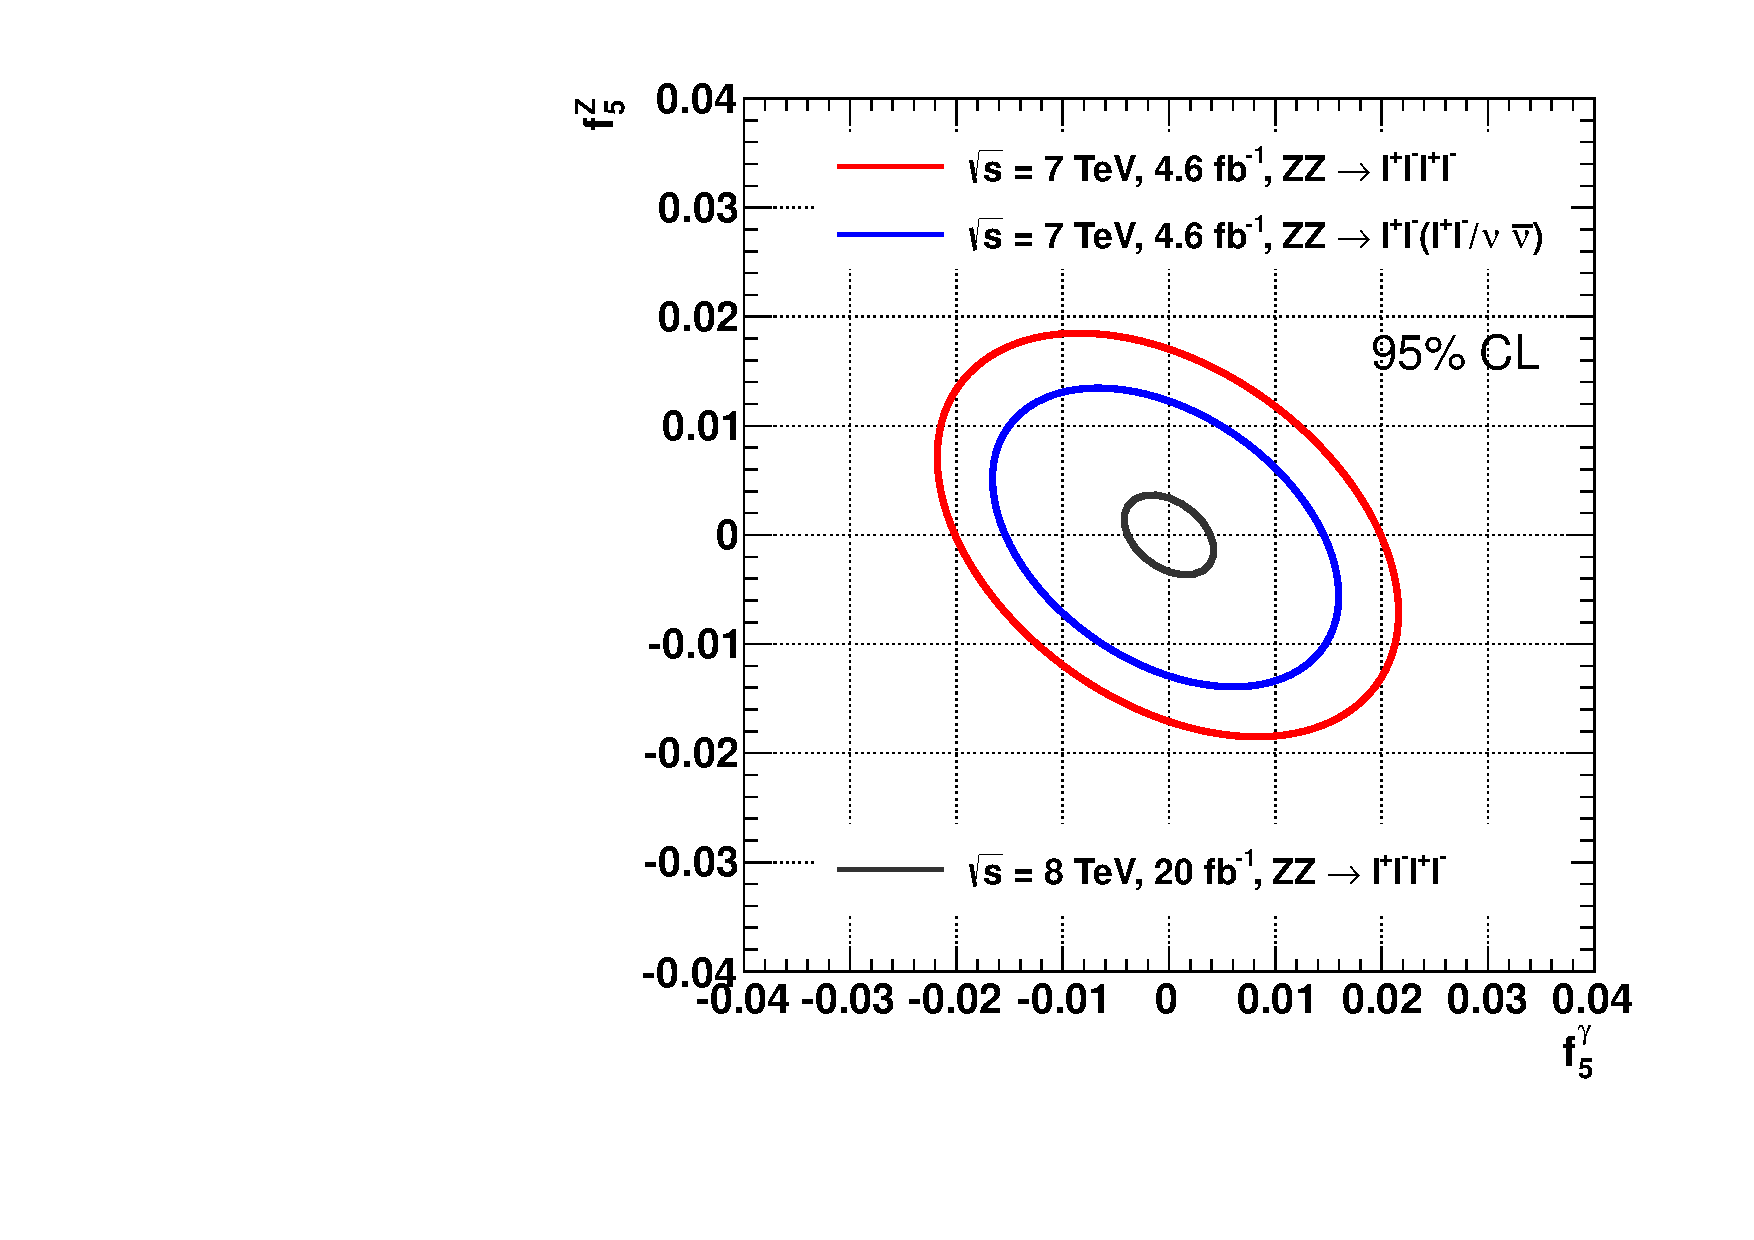
\includegraphics[width=0.43\textwidth]{2D_7TeV_8TeV/frequentist_f5Z_f5g}
}
\caption[Two dimensional 95\% confidence intervals for anomalous neutral
           gauge boson couplings (\TGC s) for form factor scale
           $\Lambda=\infty$.]{  Two dimensional 95\% confidence intervals for anomalous neutral
           gauge boson couplings (\TGC s) for form factor scale
           $\Lambda=\infty$. The limits set
           using the 7~\tev\ data using only the \ZZllll\ channel are shown in
           red, limits set using the 7~\tev\ combining the \ZZllll\ and \ZZllvv\
           channels are shown in red, and the limits obtained using the 8~\tev\
           data using only the \ZZllll\ channel are shown in black. For each pair of parameters, the other parameters
           are assumed to be fixed at their \sm\ value of zero. 
           %The one dimensional triple gauge coupling limits are 
         %shown as a projection along the axis.  
}
\label{fig:TGC-limits-2D}
\end{center}
\end{figure}

%\begin{figure}[htbp]
%\begin{center}
%%\subfigure[]{
%%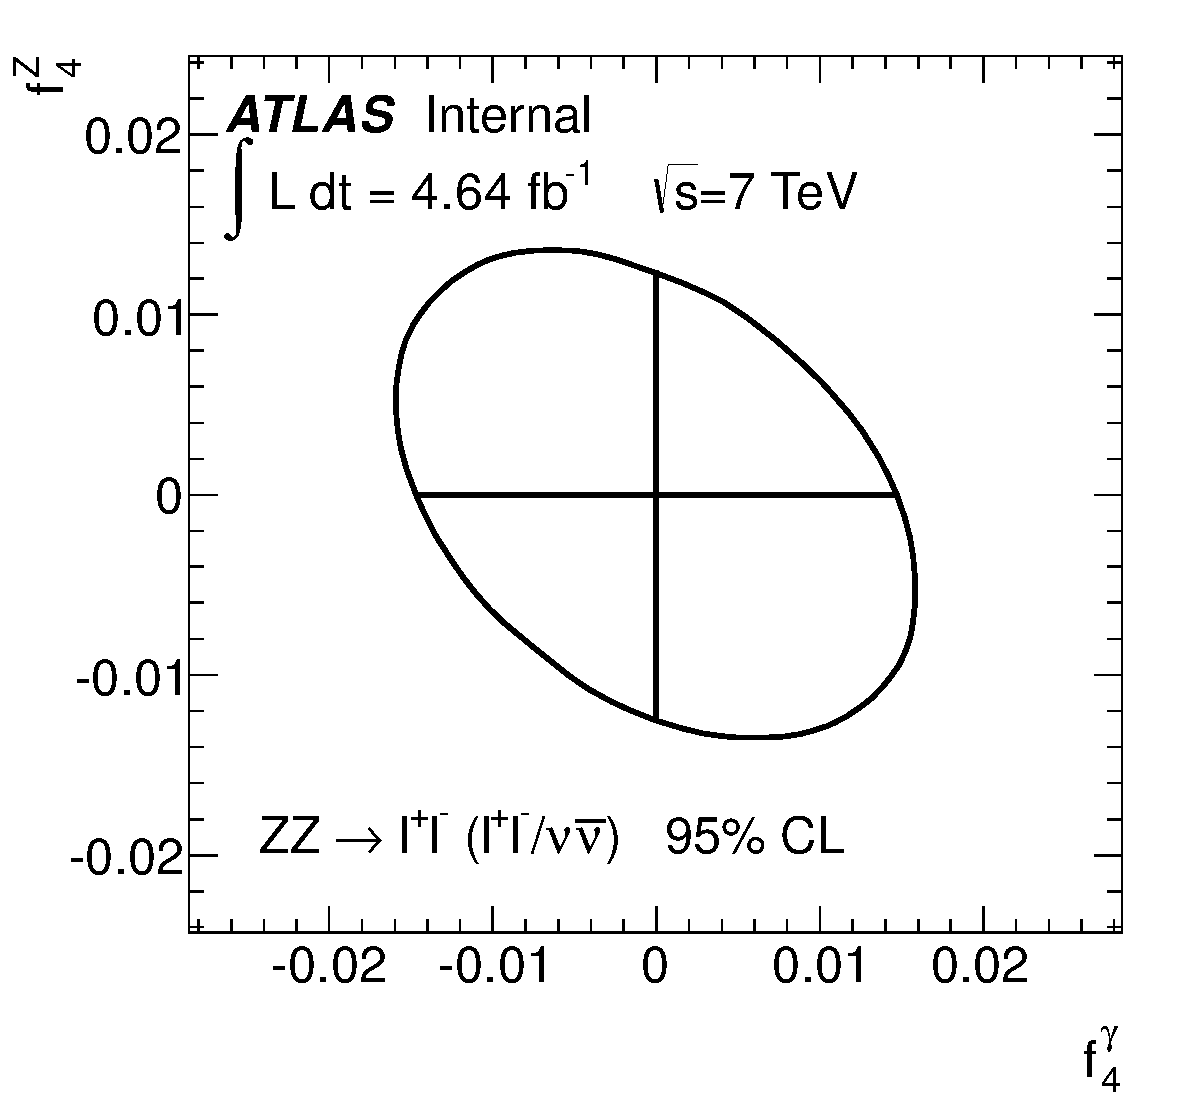
\includegraphics[width=0.43\textwidth]{2D7TeV/tgc2d_f4g_f4z}
%%}
%%\subfigure[]{
%%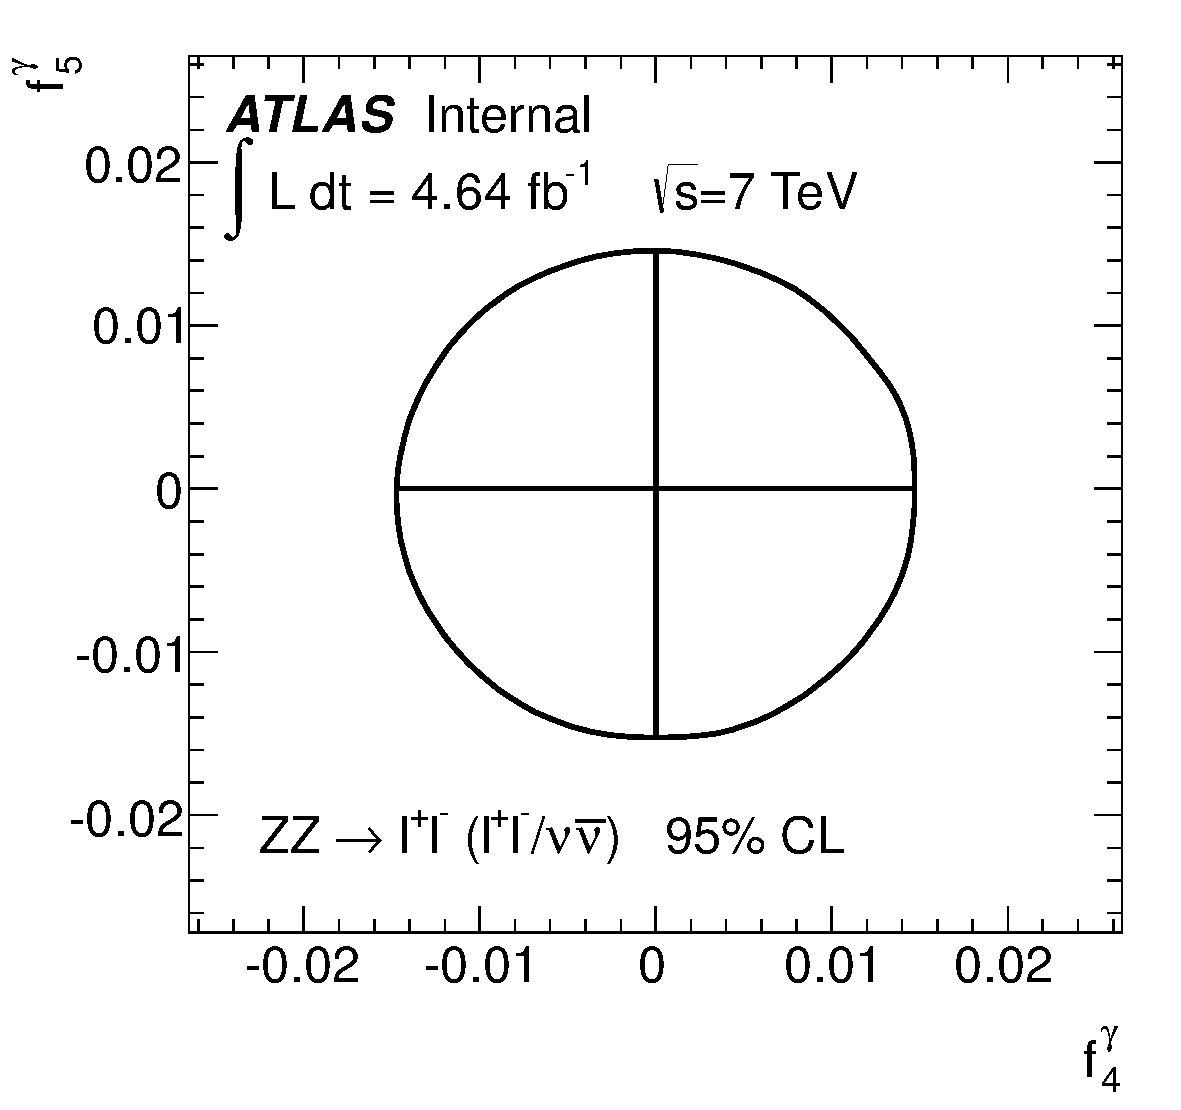
\includegraphics[width=0.43\textwidth]{2D7TeV/tgc2d_f4g_f5g}
%%}
%%\subfigure[]{
%%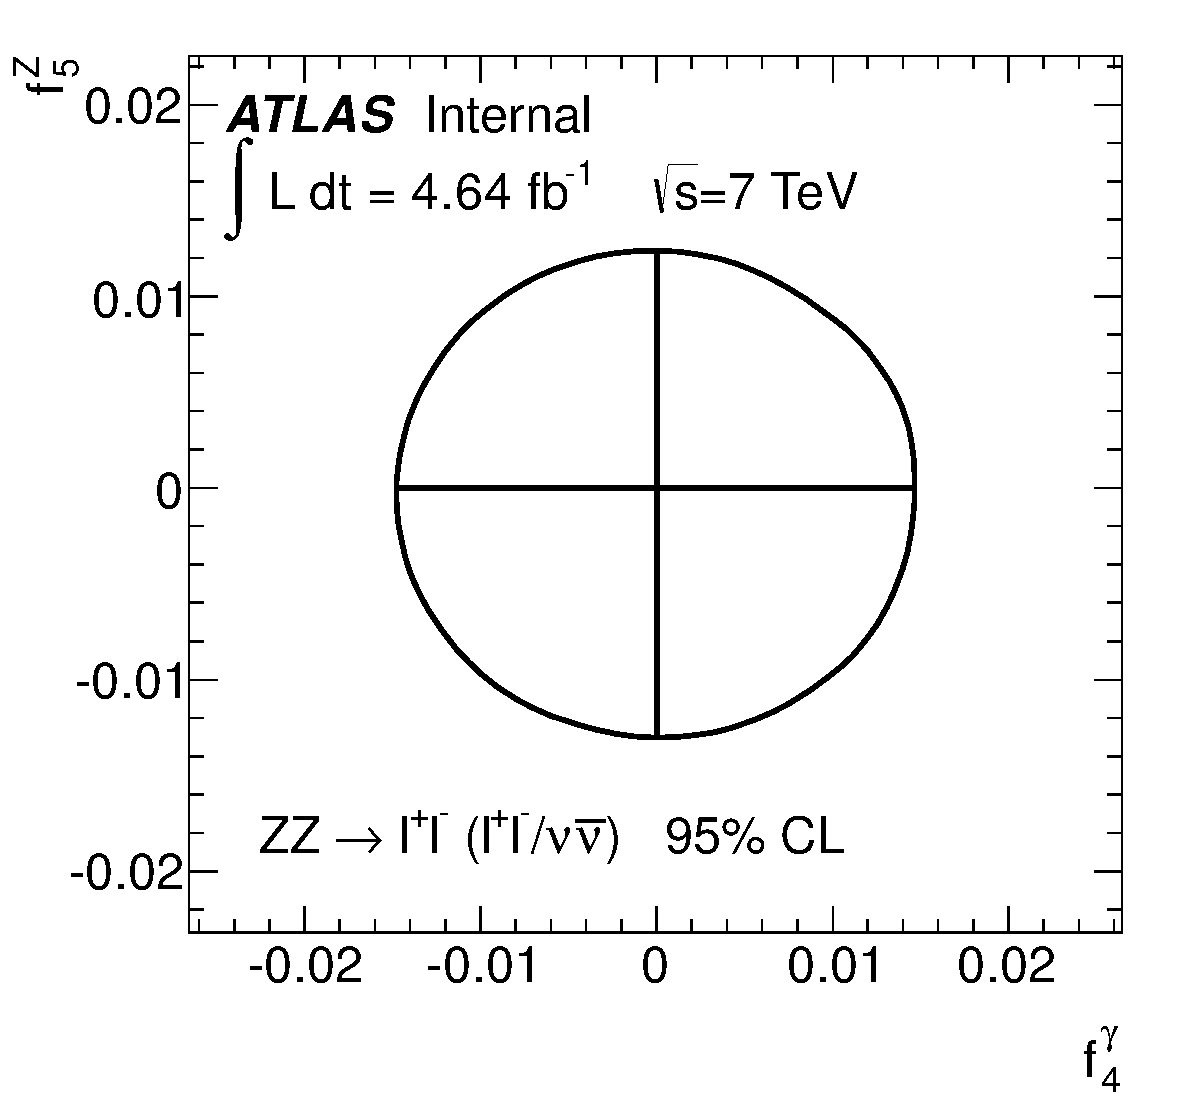
\includegraphics[width=0.43\textwidth]{2D7TeV/tgc2d_f4g_f5z}
%%}
%%\subfigure[]{
%%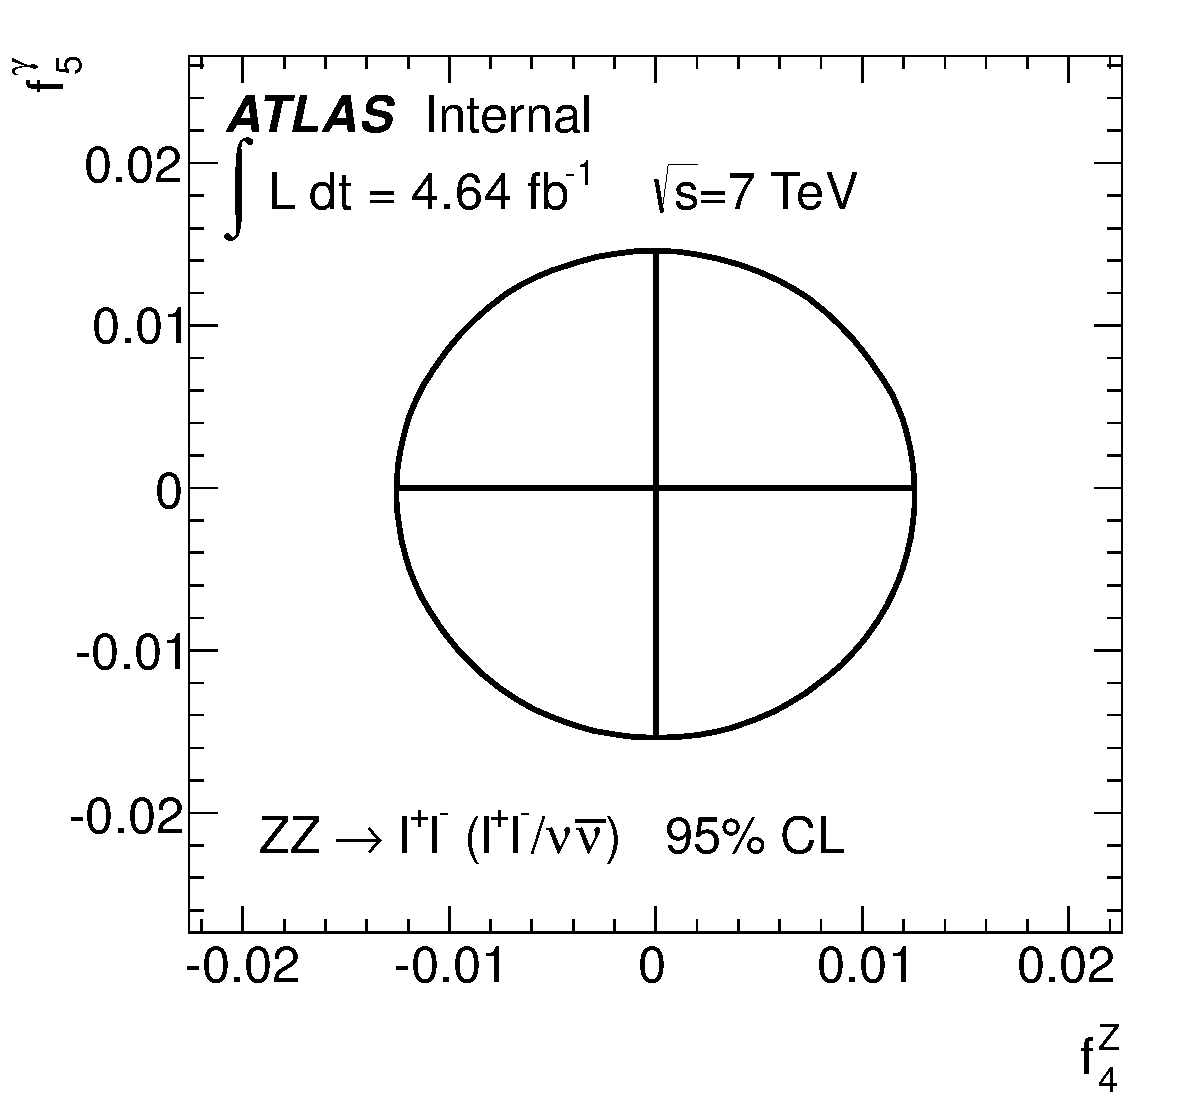
\includegraphics[width=0.43\textwidth]{2D7TeV/tgc2d_f4z_f5g}
%%}
%%\subfigure[]{
%%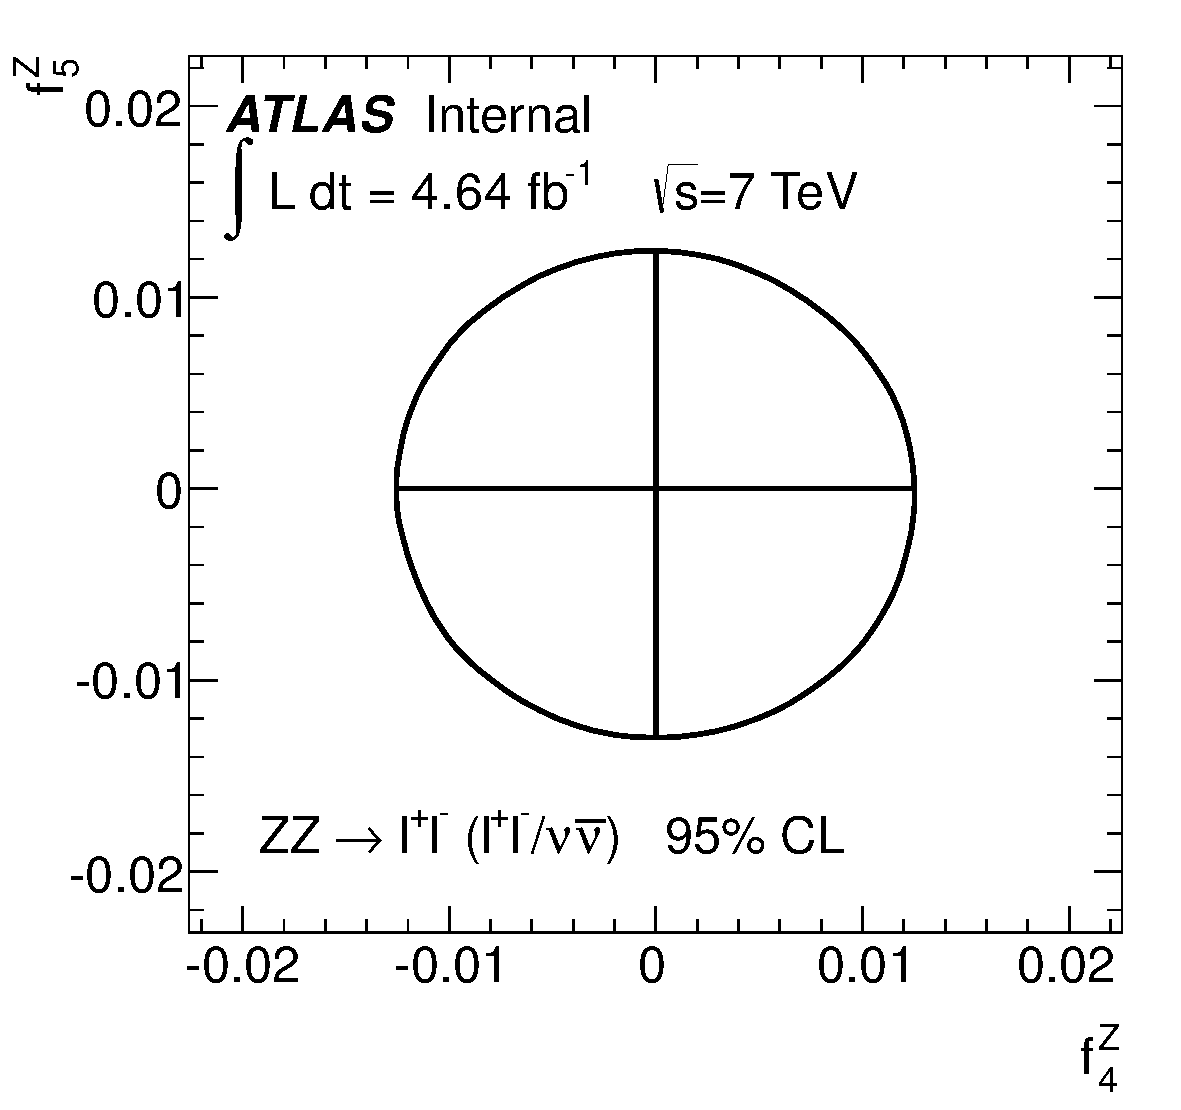
\includegraphics[width=0.43\textwidth]{2D7TeV/tgc2d_f4z_f5z}
%%}
%%\subfigure[]{
%%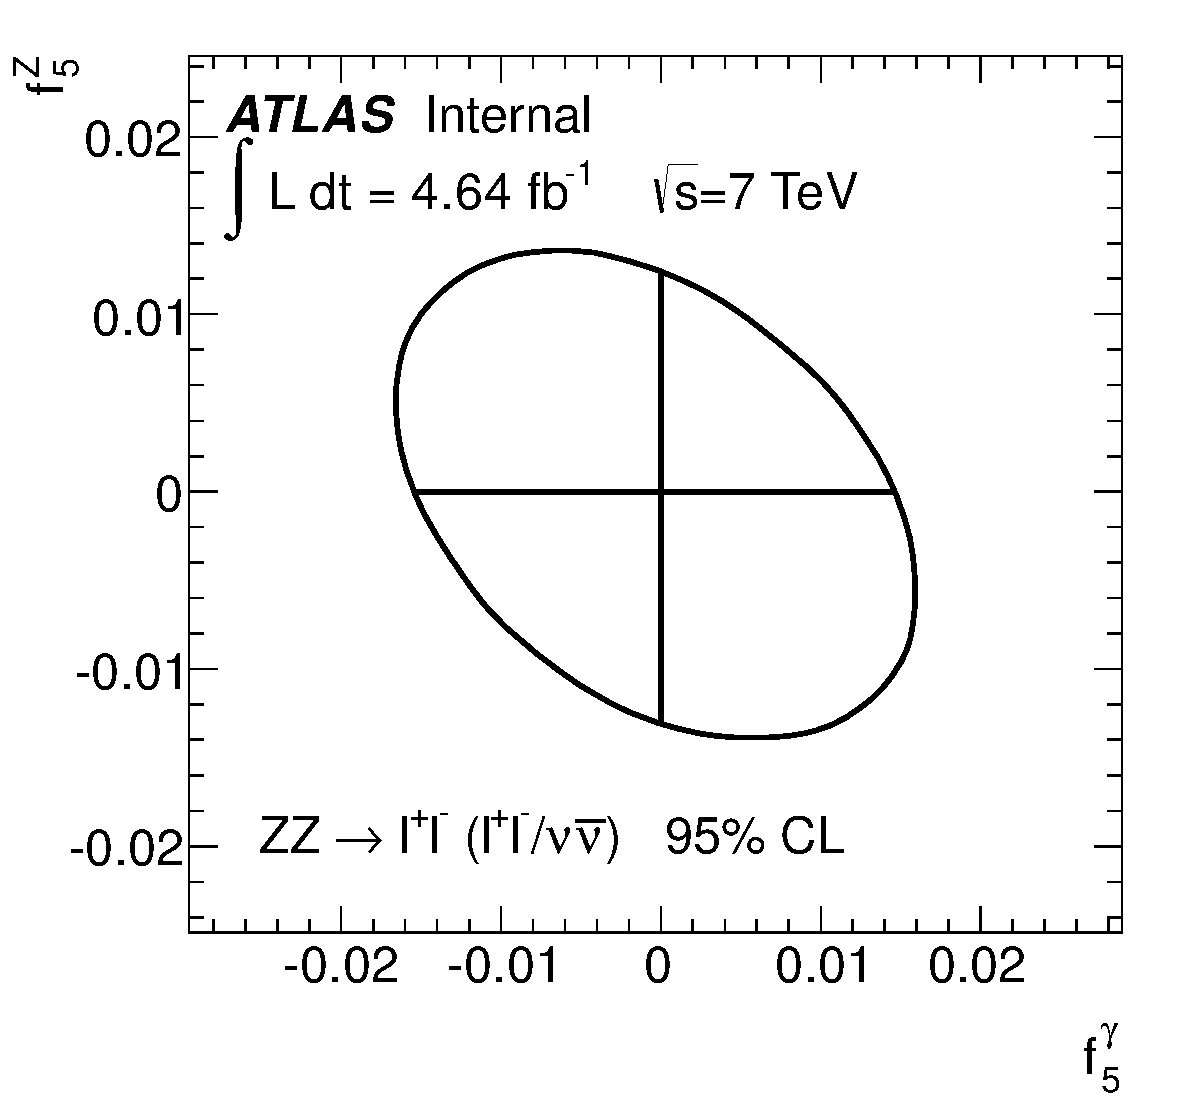
\includegraphics[width=0.43\textwidth]{2D7TeV/tgc2d_f5g_f5z}
%%}
%\caption{         Two dimensional triple gauge coupling limits for form factor scale $\Lambda=\infty$. The one dimensional triple gauge coupling limits are 
%         shown as a projection along the axis.  
%}
%\label{fig:TGC-limits-2D-eight}
%\end{center}
%\end{figure}

 \begin{figure}[htbp]
 \begin{center}
  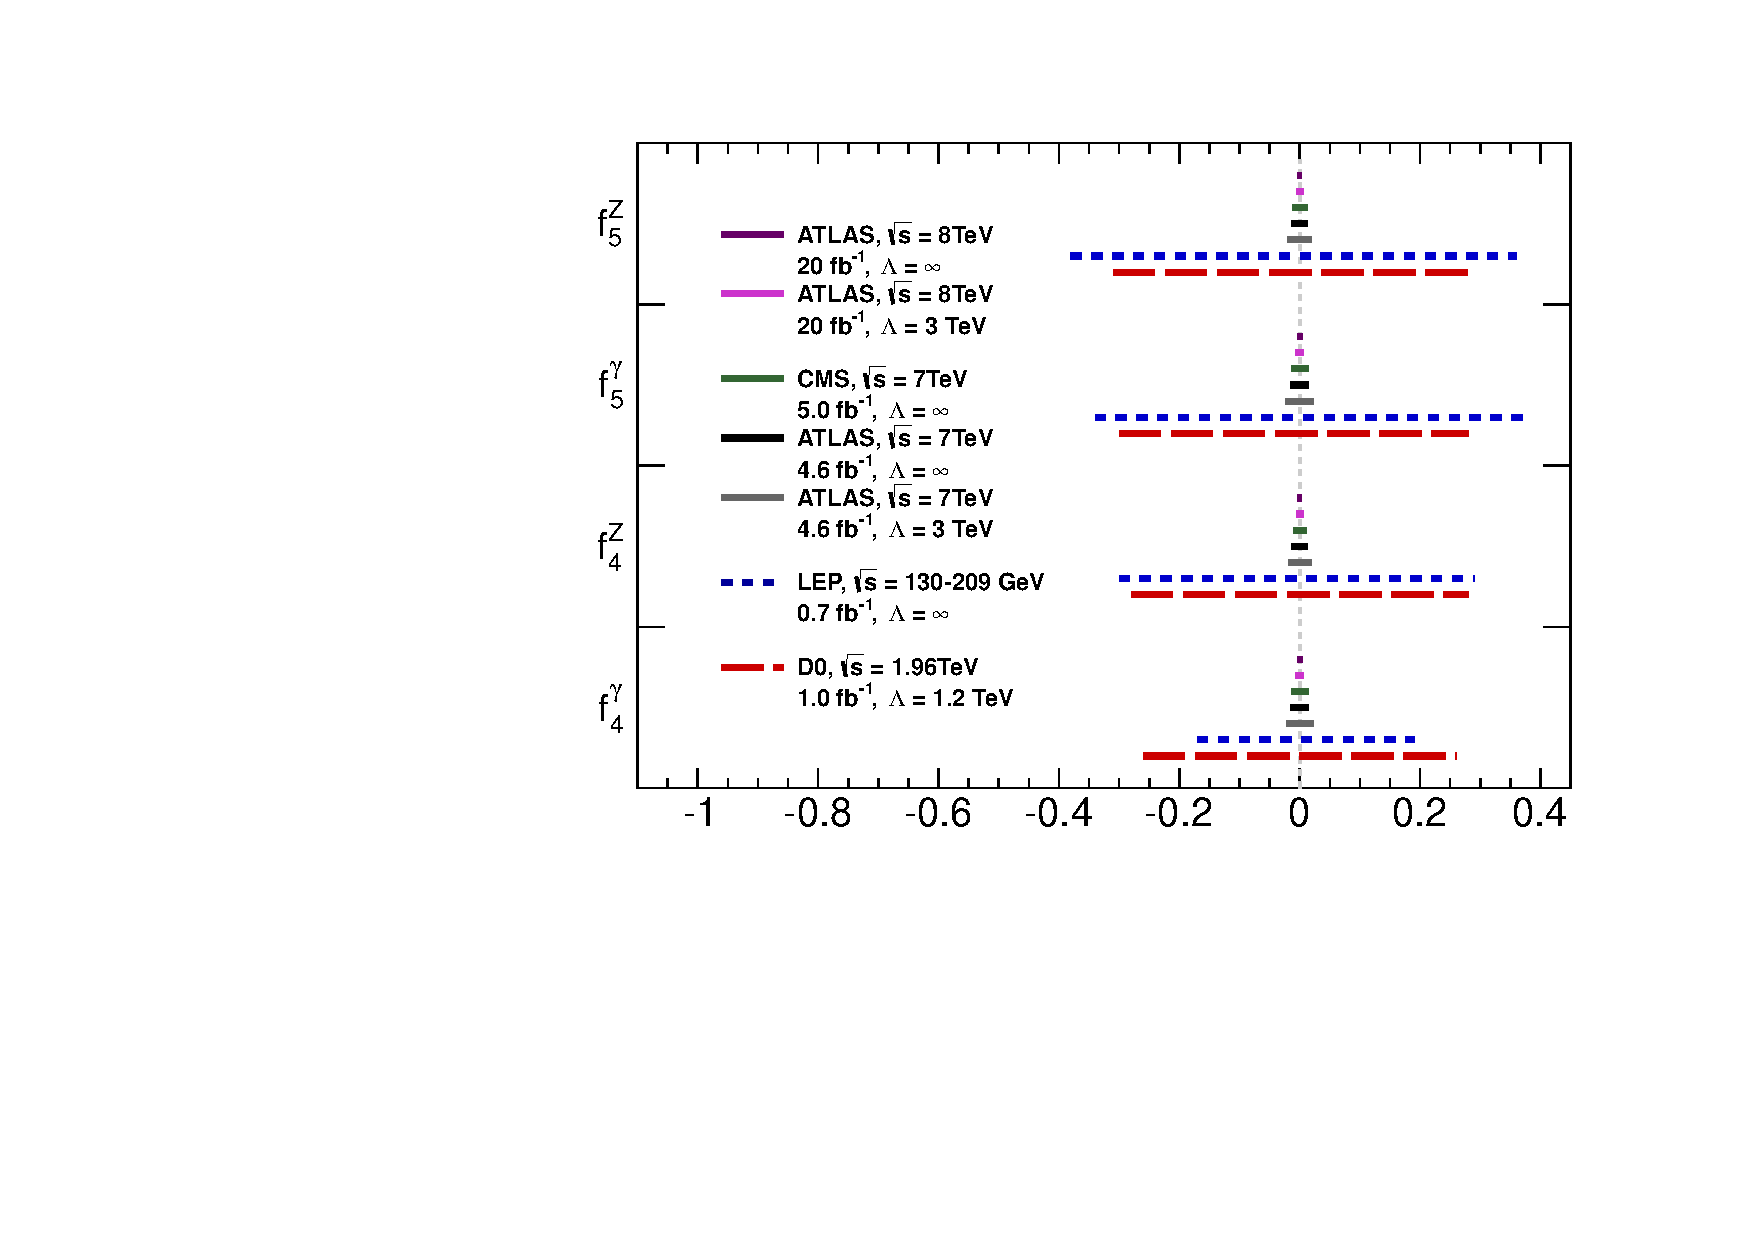
\includegraphics[width=0.9\textwidth]{SummaryPlot}\hfill
  \caption{\small 
Anomalous neutral triple gauge coupling (\TGC) 95\% confidence intervals from the ATLAS, CMS~\cite{CMS:2012rg},
LEP~\cite{bib:LEPEW2006} and Tevatron~\cite{Abazov:2007ad}
experiments. Luminosities, centre-of-mass energies and cut-offs $\Lambda$ for each experiment are shown.
   }
\label{fig:TGC-SummaryPlot}
 \end{center}
 \end{figure}
